\part*{Supplementary Material} 

\setcounter{table}{0}
\setcounter{figure}{0}
\renewcommand{\thetable}{S\arabic{table}}
\renewcommand{\thefigure}{S\arabic{figure}}

\subsection{Formula for Set Size}
To calculate the size of the different model sets, we use the binomial coefficients to calculate the number of possible combinations. The general form of the binomial coefficient is written as
\[\left( \begin{array}{c}
n \\ 
k \end{array}
\right)=\frac{n!}{k!\left(n-k\right)!}\] 

where $n$ is the number of elements which in our case is the number of covariates that we want to include, and $k$ is the number of elements taken out. $!$ is the factorial operator, so $n!=n\times \left(n-1\right)\times \left(n-2\right)\times \left(n-3\right)\times \dots \times 3\times 2\times 1$. The binomial coefficient therefore gives us the number of ways that $k$ elements can be chosen from a set of size $n$. One rule that has been repeatedly used is that we can rewrite the sum of binomial coefficients excluding the empty set i.e., not including i=0, as 
\[\sum^n_{i=1}{\left( \begin{array}{c}
n \\ 
i \end{array}
\right)}=2^n-1\] 
\\
If we include the empty set, as it is the case in some sets, this becomes
\[\sum^n_{i=0}{\left( \begin{array}{c}
n \\ 
i \end{array}
\right)}=2^n\] 
\\
When calculating the size of each set, we consider two different cases; one where we allow interactions without the corresponding main effects, and one where main effects always follow interactions. \\

\section{Case 1 – No Restriction}
\subsection{Set $x + z$}
To calculate the size of the sets, we used the binomial coefficient. The set $x + z$ will be the all the different combinations that can be made by the covariates including the model where there is only the variable of interest (based on the previous terminology also called the empty set) and the binomial coefficients can therefore give us how many of these combinations that exists. Let us denote the number of covariates with n. If we have an example with three covariates (n=3), then the combination of these where we have all three covariates present can be written using the binomial coefficient as
\[\left( \begin{array}{c}
3 \\ 
3 \end{array}
\right)=\frac{3!}{3!\left(3-3\right)!}=1\]
If only two covariates are present from the set of three covariates at the same time, then the number of possible combinations becomes 
\[\left( \begin{array}{c}
3 \\ 
2 \end{array}
\right)=\frac{3!}{2!\left(3-2\right)!}=3\] 
And the same if only one covariate is present
\[\left( \begin{array}{c}
3 \\ 
1 \end{array}
\right)=\frac{3!}{1!\left(3-1\right)!}=3\] 
Finally, where no covariates are present, the number of possible combinations is computed as follows
\[\left( \begin{array}{c}
3 \\ 
0 \end{array}
\right)=\frac{3!}{0!\left(3-0\right)!}=1\] 
The total number of models in this set will then be the sum of all these


\[\# of models\ in\ x + z = \left( \begin{array}{c}
3 \\ 
3 \end{array}
\right)+\left( \begin{array}{c}
3 \\ 
2 \end{array}
\right)+\left( \begin{array}{c}
3 \\ 
1 \end{array}
\right)+\left( \begin{array}{c}
3 \\ 
0 \end{array}
\right)=\sum^3_{i=0}{\left( \begin{array}{c}
3 \\ 
i \end{array}
\right)}\] 
Using the rule for adding binomial coefficients, we can rewrite this into
\[\# of models\ in\ x + z = \sum^3_{i=0}{\left( \begin{array}{c}
3 \\ 
i \end{array}
\right)}=\left(2^3\right)=8\] 
We can further generalize this to the n covariates case as follows 
\[\# of models\ in\ x + z\sum^n_{i=0}{\left( \begin{array}{c}
n \\ 
i \end{array}
\right)}=\left(2^n\right)\] 

\subsubsection{Formally Written} \break 
\noindent Let \emph{Z} be the set of covariates 
\[Z=\{\left.z_1,z_2,..,z_n\right.\}\] 
\[\left|Z\right|=n\] 


\noindent The $x + z$ set is then the power set of \emph{Z} 
\[x + z = \{\left.S:S\subseteq Z\right.\}\] 

Each element $S\in x + z$ is a set of the covariates (e.g., $S=\left.z_3,z_7\right.$) or any combination of the covariates, including the empty set. This is just the power set of Z and the size of the set can be written as
\[\left|x + z\right|=|\mathcal{P}\left(Z\right)|=2^n\] 

\subsection{Set $x \times z$}

The same line of reasoning goes for the $x \times z$ set as for $x + z$ set and we therefore only write it formally. Here, we just need to calculate the number of possible interactions between the variable of interest and the covariates. This set will therefore have the same size as the $x + z$ set, as there are just as many covariates as there are two-way combinations between the variable of interest and the covariates excluding the empty set.

\[I_h(Z)=\left.\left\{\{x_i,h\}\right.:x_i\in Z\right.\}\] 
\[x \times z=\left.\{T:T\subseteq I_h\left(Z\right),T\neq \textrm{\O}\right.\}\] 
The total number of models in this set is only the power set excluding the empty set
\[\left|x \times z\right|\boldsymbol{=}2^n-1\] 

\subsection{Set $z \times z$}

For the $z \times z$ set, we need the combinations of all the two-way interactions between the covariates themselves. This means we first need to calculate the possible number of two-way interactions between the interactions and thereafter the number of combinations of these interactions. If we stick to the case with n=3, then the number of combinations is as follows
\[\#\ of\ two-way\ interactions=\left( \begin{array}{c}
3 \\ 
2 \end{array}
\right)=\frac{3!}{2!\left(3-2\right)!}=3\] 
We can now make the combinations of these interaction effects. In this case $n$ does not denote the number of covariates, but the number of two-way interactions that can be made with three covariates.  

\noindent 
\[\# of models\ in\ z \times z=\left( \begin{array}{c}
3 \\ 
3 \end{array}
\right)+\left( \begin{array}{c}
3 \\ 
2 \end{array}
\right)+\left( \begin{array}{c}
3 \\ 
1 \end{array}
\right)=\sum^3_{i=1}{\left( \begin{array}{c}
3 \\ 
i \end{array}
\right)}=7\] 
In the general case, let us define the number of two-way interactions with h; this gives us
\[h=\left( \begin{array}{c}
n \\ 
2 \end{array}
\right)=n(n-1)/2\] 
So the general term for the total number of models in $z \times z$ is then
\[\# of models\ in\ z \times z=\sum^{n(n-1)/2}_{i=1}{\left( \begin{array}{c}
n(n-1)/2 \\ 
i \end{array}
\right)}=(2^{n(n-1)/2}-1)=2^h-1\] 


\subsubsection{Formally written}
Let \emph{Z} be a set of covariates 
$Z=\{z_1,z_2,..,z_n\}$
\[I_k\left(Z\right)=\{\left.\left.x_i,x_j\right.:x_i\in Z,x_j\in Z,x_i\neq x_j\right.\}\] 
\[\left|I_k\left(Z\right)\right|=\left( \begin{array}{c}
n \\ 
2 \end{array}
\right)=\frac{n\left(n-1\right)\left(n-2\right)!}{\left(n-2\right)!}\frac{1}{2}=n(n-1)/2\] 
The set of all combinations of the different interactions between the covariates is then all the subsets of $I_k\left(Z\right)$ excluding the empty set
\[P\left(I_k\left(Z\right)\right)=\{\left.J:J\subseteq I_k\left(Z\right),J\neq \textrm{\O}\right.\}\] 
\[\left|z \times z\right|=\left|P\left(I_k\left(Z\right)\right)\right|=2^{\left|I_k\left(Z\right)\right|}-1=2^{n(n-1)/2}-1\] 
defining 
\[h=\left( \begin{array}{c}
n \\ 
2 \end{array}
\right)=n(n-1)/2\] \\
so we can write the number of models in $z \times z$ as
\[\left|z \times z\right|=2^h-1\] \\

\subsection{Full model set}
For the following sets: $x + z + x \times z$ , $x + z + z \times z$, and $x + z + x \times z$ + $z \times z$, the math follows directly from the previous equations as these sets are the product of the previously calculated sets. 

\[\# of models\ in\ x + z\left(2^n\right)\] 
\[\# of models\ in\ x \times z=\left(2^n-1\right)\] 
\[\# of models\ in\ z \times z=\left(2^h-1\right)\] 
\[\# of models\ in\ x + z + x \times z={\left(2^n-1\right)}^2\] 
\[\# of models\ in\ x + z+z \times z=\left(2^n-1\right)\left(2^h-1\right)\] 
\[\# of models\ in\ x + z + x \times z+z \times z={\left(2^n-1\right)}^2\left(2^h-1\right)\] 
So the total number of models including all sets then becomes
\begin{equation*}
\begin{aligned}
$total \# of models=\\
& \underbrace{\left(2^n\right)}_{x + z}+\underbrace{\left(2^n-1\right)}_{x \times z}+\underbrace{\left(2^h-1\right)}_{z \times z}+\\
&\underbrace{{\left(2^n-1\right)}^2}_{x + z + x \times z}+\underbrace{\left(2^n-1\right)\left(2^h-1\right)}_{x \times z+z \times z}+\underbrace{\left(2^n-1\right)\left(2^h-1\right)}_{x + z+z \times z}+\\
&\underbrace{{\left(2^n-1\right)}^2\left(2^h-1\right)}_{x + z + x \times z+z \times z}$ 
\end{aligned}
\end{equation*}

For the case where n=2, (as in Table S1), this gives us
\[h=\left( \begin{array}{c}
2 \\ 
2 \end{array}
\right)=1\] 
\[\total \# of models=\left(2^2\right)+\left(2^2-1\right)+\left(2^1-1\right)+{\left(2^2-1\right)}^2+2\left(2^2-1\right)\left(2^1-1\right)+{\left(2^2-1\right)}^2\left(2^1-1\right)=32\] 

\begin{table}[hbt!]
\caption{}
\caption*{\footnotesize Overview of all models per each model set when there are two covariates and one dependent variable}
\centering
\begin{tabular}{cc}
\toprule
Model set & Models \\  
\midrule
\multirow{4}{*}{x + z} & $y=x_1$ \\ & $y=x_1+z_1$ \\ & $y=x_1+z_2$ \\ & $y=x_1+z_1+z_2$ & \\ 
\multirow{3}{*}{$x \times z$} & $y=x_1+x_1z_1$ \\ & $y=x_1+x_1z_2$ \\ & $y=x_1+x_1z_1+x_1z_2$ & \\
$z \times z$ & $y=x_1+z_1z_2$ & \\ 
\multirow{9}{*}{$x + z + x \times z$} & $y=x_1+z_1+x_1z_1$\\ & $y=x_1+z_1+x_1z_2$\\ & $y=x_1+z_1+x_1z_1+x_1z_2$\\ & $y=x_1+z_2+x_1z_1$\\ & $y=x_1+z_2+x_1z_2$\\ & $y=x_1+z_2+x_1z_1+x_1z_2$\\ & $y=x_1+z_1+z_2+x_1z_1$\\ & $y=x_1+z_1+z_2+x_1z_2$\\ & $y=x_1+z_1+z_2+x_1z_1+x_1z_2$ & \\ 
\multirow{3}{*}{$x + z + z \times z$} & $y=x_1+z_1+z_1z_2$\\ & $y=x_1+z_2+z_1z_2$\\ & $y=x_1+z_1+z_2+z_1z_2$ & \\
\multirow{3}{*}{$x \times z + z \times z$} & $y=x_1+x_1z_1+z_1z_2$\\ & $y=x_1+x_1z_2+z_1z_2$\\ & $y=x_1+x_1z_1+x_1z_2+z_1z_2$ & \\
\multirow{9}{*}{$x + z + x \times z + z \times z$} & $y=x_1+z_1+x_1z_1+z_1z_2$\\ & $y=x_1+z_1+x_1z_2+z_1z_2$\\ & $y=x_1+z_1+x_1z_1+x_1z_2+z_1z_2$\\ & $y=x_1+z_2+x_1z_1+z_1z_2$\\ & $y=x_1+z_2+x_1z_2+z_1z_2$\\ & $y=x_1+z_2+x_1z_1+x_1z_2+z_1z_2$\\ & $y=x_1+z_1+z_2+x_1z_1+z_1z_2$\\ & $y=x_1+z_1+z_2+x_1z_2+z_1z_2$\\ & $y=x_1+z_1+z_2+x_1z_1+x_1z_2+z_1z_2$ \\ 
\bottomrule
\end{tabular}
\end{table}
\newpage
\section{Case 2 – With Restriction}

In this case, we need to ensure that every time there is an interaction, the main effects follow. This means that if the variable of interest interacts with a covariate, both the variable of interest and the covariate will be present as the main effects, e.g.,
\[y=x_1+z_1+x_1z_1\] 

In the previous equation, we have an interaction between our variable of interest $x_1$ and a covariate $z_1$. Therefore, the two corresponding main effects also enter the model. This restriction does not change how we calculate the set size of the $x + z$ set as there are no interactions in it. The way to calculate the size of the $x + z$ set is therefore the same in the two cases (i.e., with and without restriction); we will therefore focus on calculating the other set sizes. However, having a restriction that main effects should always follow interactions means that we need to exclude the models from the $x \times z$ and $z \times z$ sets as these do not have main effect following interactions. The first set we then need to calculate is the $x + z + x \times z$ set.

\subsection{$x + z + x \times z$}
For the sake of simplicity, we start with a case where n=3. The models that are within this set can be seen in Table S2. \\

\begin{table}[hbt!]
\caption{}
\caption*{Overview of the models in the $x + z + x \times z$ set when there are three covariates and one dependent variable}
\centering
\begin{tabular}{cc}
\toprule
Model set & Models \\ 
\midrule
\multirow{19}{*}{$x + z + x \times z$} & $y=x_1+z_1+x_1z_1$\\ &  $y=x_1+z_2+x_1z_2$\\ &  $y=x_1+z_3+x_1z_3$\\ & $y=x_1+z_1+z_2+x_1z_1$\\ & $y=x_1+z_1+z_3+x_1z_1$\\ & $y=x_1+z_3+z_1+x_1z_3$\\ & $y=x_1+z_3+z_2+x_1z_3$\\ & $y=x_1+z_2+z_1+x_1z_2$\\ & $y=x_1+z_2+z_3+x_1z_2$\\ & $y=x_1+z_1+z_2+z_3+x_1z_1$\\ & $y=x_1+z_1+z_2+z_3+x_1z_2$\\ & $y=x_1+z_1+z_2+z_3+x_1z_3$\\ & $y=x_1+z_1+z_2+x_1z_1+x_1z_2$\\ & $y=x_1+z_1+z_3+x_1z_1+x_1z_3$\\ & $y=x_1+z_1+z_2+x_1z_3+x_1z_2$\\ & $y=x_1+z_1+z_2+z_3+x_1z_1+x_1z_2$\\ & $y=x_1+z_1+z_2+z_3+x_1z_1+x_1z_3$\\ & $y=x_1+z_1+z_2+z_3+x_1z_3+x_1z_2$\\ & $y=x_1+z_1+z_2+z_3+x_1z_1+x_1z_2+x_1z_3$\\  
\bottomrule
\end{tabular}
\end{table}

In Table S3, we divided the $x + z + x \times z$ set into three parts - $x + z + x \times z$(1), $x + z + x \times z$(2), and $x + z + x \times z$(3) - which contain all the models where there are one, two, or three covariates, respectively. \\

\begin{table}[hbt!]
\caption{Split of the $x + z + x \times z$ set into three subsets when there are three covariates and one dependent variable. $x + z + x \times z$(1) is all the models with one covariate as main effect, $x + z + x \times z$(2) is all the models with two covariates as main effects, and $x + z + x \times z$(3) is all the models with three covariates as main effects}
\centering
\begin{tabular}{lc}  
\toprule
Set & Models \\
\midrule
\multirow{3}{*}{$x + z + x \times z$(1)} & $y=x_1+z_1+x_1z_1$\\ & $y=x_1+z_2+x_1z_2$\\ & $y=x_1+z_3+x_1z_3$\\ & \\ 
\multirow{9}{*}{$x + z + x \times z$(2)} & $y=x_1+z_1$$+z_2+x_1z_1$\\ & $y=x_1+z_1+z_3+x_1z_1$\\ & $y=x_1+z_3+z_1+x_1z_3$\\ & $y=x_1+z_3+z_2+x_1z_3$\\ & $y=x_1+z_2+z_1+x_1z_2$\\ & $y=x_1+z_2+z_3+x_1z_2$\\ & $y=x_1+z_1+z_2+x_1z_1+x_1z_2$\\ & $y=x_1+z_1+z_3+x_1z_1+x_1z_3$\\ & $y=x_1+z_1+z_2+x_1z_3+x_1z_2$\\  & \\  
\multirow{7}{*}{$x + z + x \times z$(3)} & $y=x_1+z_1+z_2+z_3+x_1z_1$\\ & $y=x_1+z_1+z_2+z_3+x_1z_2$\\ & $y=x_1+z_1+z_2+z_3+x_1z_3$\\ & $y=x_1+z_1+z_2+z_3+x_1z_1+x_1z_2$\\ & $y=x_1+z_1+z_2+z_3+x_1z_1+x_1z_3$\\ & $y=x_1+z_1+z_2+z_3+x_1z_3+x_1z_2$\\ & $y=x_1+z_1+z_2+z_3+x_1z_1+x_1z_2+x_1z_3$\\  
\bottomrule
\end{tabular}
\end{table}

To calculate the size of each of these sets separately, we only need to focus on the number of covariates that enters the model, as per assumption the variable of interest $x_1$ is always present. Let us start with the $x + z + x \times z$(1) set. In this set, there can only be one covariate present at the same time; there are therefore three combinations, which can be written as $\binom{3}{1}$. In this set, since there is only one covariate, there is only one interaction term containing that same covariate. As there can be made no other combinations, this corresponds to $\binom{1}{1}$. Using the same shorthand notation with the binomial coefficient as so far, we can write the number of models in the $x + z + x \times z$(1) set as
\[\#\ of\ models\ in\ x + z + x \times z\textit{(1)}\ =\left( \begin{array}{c}
1 \\ 
1 \end{array}
\right)\left( \begin{array}{c}
3 \\ 
1 \end{array}
\right)=\sum^1_{i=1}{\left( \begin{array}{c}
1 \\ 
i \end{array}
\right)}\left( \begin{array}{c}
3 \\ 
1 \end{array}
\right)=\left(2^1-1\right)\left( \begin{array}{c}
3 \\ 
1 \end{array}
\right)=3\] 

Using this notation for the formulation makes sense when we have to combine the three sets of $x + z + x \times z$ into one to calculate all the models in $x + z + x \times z$.

For the $x + z + x \times z$(2) set, we first need to calculate the number of combinations for the main effect that can be made when there are two covariates present at all times and that is $\binom{3}{2}$. Next we need to calculate the number of combinations of interactions that can be present. As we have two covariates present all the time, these are the ones that can be used in the interaction effects. Since the covariates interact with $x_1$, there can either be one or two interaction effects present. Hence, we have $\binom{2}{1}$ and $\binom{2}{2}$ combinations of the interaction effects possible. Combining the number of covariates with the number of possible interactions we get
\begin{equation*}
\begin{aligned}
\#\ of\ models\ in\ x + z +x \times z\textit{(2)}=\\
& \left( \begin{array}{c}
2 \\ 
1 \end{array}
\right)\left( \begin{array}{c}
3 \\ 
2 \end{array}
\right)+\left( \begin{array}{c}
2 \\ 
2 \end{array}
\right)\left( \begin{array}{c}
3 \\ 
2 \end{array}
\right)=\\
&\sum^2_{i=1}{\left( \begin{array}{c}
2 \\ 
i \end{array}
\right)}\left( \begin{array}{c}
3 \\ 
2 \end{array}
\right)=\left(2^2-1\right)\left( \begin{array}{c}
3 \\ 
2 \end{array}
\right)=9

\end{aligned}
\end{equation*}
The same reasoning goes for the $x + z + x \times z$(3) set; the only difference here is that we have one more covariate. So if we write the combinations that are possible with three covariates in the same way as before, we get
\begin{equation*}
\begin{aligned}
\#\ of\ models\ in\ x + z + x \times z\textit{(3)}=\\
&\left( \begin{array}{c}
3 \\ 
1 \end{array}
\right)\left( \begin{array}{c}
3 \\ 
3 \end{array}
\right)+\left( \begin{array}{c}
3 \\ 
2 \end{array}
\right)\left( \begin{array}{c}
3 \\ 
3 \end{array}
\right)+\left( \begin{array}{c}
3 \\ 
3 \end{array}
\right)\left( \begin{array}{c}
3 \\ 
3 \end{array}
\right)= \\
&\sum^3_{i=1}{\left( \begin{array}{c}
2 \\ 
i \end{array}
\right)}\left( \begin{array}{c}
3 \\ 
2 \end{array}
\right)= \\
&\left(2^3-1\right)\left( \begin{array}{c}
3 \\ 
3 \end{array}
\right)=7
\end{aligned}
\end{equation*}


We can then sum all three sets that is, $x + z + x \times z$(1), $x + z + x \times z$(2) and $x + z + x \times z$(3), to get the size of the $x + z + x \times z$ set
\[\#\ of\ models\ in\ $x + z + x \times z$=\sum^3_{k=1}{(2^k-1)\left( \begin{array}{c}
3 \\ 
k \end{array}
\right)}\] where k is the number of covariates that goes in as main effects, meaning it is an indicator for $x + z + x \times z$(1), $x + z + x \times z$(2) and $x + z + x \times z$(3).
For the case with n covariates, this becomes
\[\#\ of\ models\ in\ x + z + x \times z=\sum^n_{k=1}{(2^k-1)\left( \begin{array}{c}
n \\ 
k \end{array}
\right)}\] 

\subsubsection{Formally written}
Let $Z$ be a set of covariates 
\[Z=\{\left.z_1,z_2,\dots ,z_n\right.\}\] 
\[|Z|=n\] 

Let J be a set of indicators of how many covariates goes into the model set as main effects
\[J=\{\left.1,2,3,4,\dots ,n\right.\}\] 
Let L be a subset of Z of size k.
\[L=\{\left.S:S\subset Z,\left|S\right|=k,k\in J\right.\}\] 

The number of interactions that can be made between a covariate and the variable of interest for a given k is then
\[I_h\left(Z\right)=\{\left.\left.x_i,x_1\right.:x_i\in L\right.\}\] 
\[\left|I_h\left(Z\right)\right|=k\] 

For each k, the number of interactions is just the power set of Z excluding the empty set
\[\left|\mathcal{P}\left(I_h\left(Z\right):I_h\left(Z\right)\neq \textrm{\O}\right)\right|=2^k-1\] 

For each k, there is $\left( \begin{array}{c}
n \\ 
k \end{array}
\right)$ combinations of interactions that can be present with the number of covariates k. To get the full set, we need to sum over these combinations from $k=1$ (with $k=0$ it would not be possible to make any interactions so this one is excluded) to $n$.
\[\left|x + z + x \times z\right|=\sum^n_{k=1}{\left( \begin{array}{c}
n \\ 
k \end{array}
\right)\left(2^k-1\right)}\] 
\textbf{}

\subsection{$x + z + z \times z$}

Here we can use the same line of reasoning as we did for the $x + z + x \times z$ set. Let us begin by looking at the $n=3$ case and then develop a more general notion from there. This example can be seen in Table S4. 
\begin{table}{}
\centering
\caption{Models for the set $x + z + z \times z$ that can be made with three covariates.}
\begin{tabular}{lc} \hline
\toprule
Set & Models \\
\midrule
\multirow{9}{*}{$x + z + z \times z$} & $y=x_1+z_1+z_2+z_1z_2$\\ & $y=x_1+z_1+z_3+z_1z_3$\\ & $y=x_1+z_2+z_3+z_2z_3$\\ & $y=x_1+z_1+z_2+z_3+z_1z_2$\\ & $y=x_1+z_1+z_3+z_2+z_1z_3$\\ & $y=x_1+z_2+z_3+z_1+z_2z_3$\\ & $y=x_1+z_1+z_2+z_3+z_1z_2+z_1z_3$\\ & $y=x_1+z_1+z_3+z_2+z_1z_3+z_2z_3$\\ & $y=x_1+z_2+z_3+z_1+z_1z_2+z_2z_3$ \\
\bottomrule
\end{tabular}
\end{table}
To make it easier to understand how to calculate the set size, we can split this set into subsets as we did before for the $x + z + x \times z$ set. This can be seen in Table S5.

\begin{table}
\centering
\caption{Split of the $x + z + z \times z$ set into two subsets when there are three covariates and one dependent variable. $x + z + z \times z$(2) is all the models with two covariates as main effects, and $x + z + z \times z$(3) is all the models with three covariates as main effects. $x + z + z \times z$(1) is not possible as you need at least two covariates to make an interaction.}
\begin{tabular}{lc} 
\toprule
Set & Models \\ 
\midrule
\multirow{3}{*}{$x + z + z \times z$(2)} & $y=x_1+z_1+z_2+z_1z_2$\\ & $y=x_1+z_1+z_3+z_1z_3$\\ & $y=x_1+z_2+z_3+z_2z_3$\\ &  \\  
\multirow{7}{*}{$x + z + z \times z$(3)} & $y=x_1+z_1+z_2+z_3+z_1z_2$\\ & $y=x_1+z_1+z_3+z_2+z_1z_3$\\ & $y=x_1+z_2+z_3+z_1+z_2z_3$\\ & $y=x_1+z_1+z_2+z_3+z_1z_2+z_1z_3$\\ & $y=x_1+z_1+z_3+z_2+z_1z_3+z_2z_3$\\ & $y=x_1+z_2+z_3+z_1+z_1z_2+z_2z_3$\\ & $y=x_1+z_1+z_2+z_3+z_1z_2+z_2z_3+z_1z_3$\\ & \\ 
\bottomrule
\end{tabular}
\end{table}

In this case, we always need to have at least two covariates present for this set to fulfil the restriction that main effects must be present as soon as there are interactions. Therefore, we can only divide the $x + z + z \times z$ set into two subsets; the first subset has two covariates present as main effects and the second subset has three covariates present as main effects. The first set, $x + z + z \times z$(2), is straightforward as this set is only the number of combinations of the three covariates that can be made when there has to be two present, meaning $\binom{3}{2}$, multiplied with the combinations of two of these covariates that are included, meaning $\binom{2}{2}$.

\noindent 
\[\#\ of\ models\ in\ x + z + z \times z\textit{(2)} =\left( \begin{array}{c}
3 \\ 
2 \end{array}
\right)\left( \begin{array}{c}
2 \\ 
2 \end{array}
\right)=3\] 

For the second subset, $x + z + z \times z$(3), the first term is the number of combinations that can be made with three covariates so this is just $\binom{3}{3}$. We then have to calculate the number of interactions that can be made with the three included covariates. To do that, first we need to calculate the number of two-way interactions that can be made with three covariates and this is just $\binom{3}{2}=3$. The total number of models in the set is then the sum of the number of combinations
\[\#\ of\ models\ in\ $x + z + z \times z$\textit{(3)}=\left( \begin{array}{c}
3 \\ 
3 \end{array}
\right)\left(\left( \begin{array}{c}
3 \\ 
1 \end{array}
\right)+\left( \begin{array}{c}
3 \\ 
2 \end{array}
\right)+\left( \begin{array}{c}
3 \\ 
3 \end{array}
\right)\right)=\left( \begin{array}{c}
3 \\ 
3 \end{array}
\right)\sum^3_{i=1}{\left( \begin{array}{c}
3 \\ 
i \end{array}
\right)}\] 

However, it is only in our example that we sum to $n=3$. In general, this will be the number of pairs that can be made in this subset. The number of pairs can be written as $\left( \begin{array}{c}
n \\ 
2 \end{array}
\right)=\frac{n\left(n-1\right)}{2}$. This then becomes
\[\#\ of\ models\ in\ x + z + z \times z\textit{(3)}=\left( \begin{array}{c}
3 \\ 
3 \end{array}
\right)\sum^3_{i=1}{\left( \begin{array}{c}
3 \\ 
i \end{array}
\right)}=\left( \begin{array}{c}
3 \\ 
3 \end{array}
\right)\sum^{\frac{3\left(3-1\right)}{2}}_{i=1}{\left( \begin{array}{c}
\frac{3\left(3-1\right)}{2} \\ 
i \end{array}
\right)}=\left( \begin{array}{c}
3 \\ 
3 \end{array}
\right)\left(2^{\frac{3\left(3-1\right)}{2}}-1\right)\] 
We can write the first subset in the same way
\[\#\ of\ models\ in\ x + z + z \times z(2)=\left( \begin{array}{c}
3 \\ 
2 \end{array}
\right)=\left( \begin{array}{c}
3 \\ 
2 \end{array}
\right)\left(2^{\frac{2\left(2-1\right)}{2}}-1\right)\] 
Now we just add these two subsets up
\[\#\ of\ models\ in\ x + z + z \times z=\left( \begin{array}{c}
3 \\ 
2 \end{array}
\right)\left(2^{\frac{2\left(2-1\right)}{2}}-1\right)+\left( \begin{array}{c}
3 \\ 
3 \end{array}
\right)\left(2^{\frac{3\left(3-1\right)}{2}}-1\right)=\sum^3_{j=2}{\left( \begin{array}{c}
3 \\ 
j \end{array}
\right)\left(2^{\frac{j\left(j-1\right)}{2}}-1\right)}\] 
We can then generalize this case for \textit{n} covariates
\[\#\ of\ models\ in\ x + z+z \times z=\sum^n_{j=2}{\left( \begin{array}{c}
n \\ 
j \end{array}
\right)\left(2^{\frac{j\left(j-1\right)}{2}}-1\right)}\] 

\subsubsection{Formally written}
Let $Z$ be a set of covariates 
\[Z=\{\left.z_1,z_2,\dots ,z_n\right.\}\] 
\[|Z|=n\] 

Let k be an indicator of how many covariates are included. Since we are using interactions, k must start at two. Let T be a set of indicators of the number of covariates starting from two
\[T=\{\left.2,3,4,\dots ,n\right.\}\] 
Let L be a subset of Z of size k.
\[L=\{\left.S:S\subset Z,\left|S\right|=k,k\in T\right.\}\] 

\noindent The number of interactions that can be made for a given k is then
\[I_k\left(Z\right)=\{\left.\left.x_i,x_j\right.:x_i\in L,x_j\in L,x_i\neq x_j\right.\}\] 
For a given k, the number of two-way interactions that can be made is then
\[\left|I_k\left(Z\right)\right|=\left( \begin{array}{c}
k \\ 
2 \end{array}
\right)=\frac{k!}{2!\left(k-2\right)!}=\frac{k\left(k-1\right)\left(k-2\right)!}{\left(k-2\right)!}\frac{1}{2}=\frac{k\left(k-1\right)}{2}\] 

We then need the combinations of all the two-way interactions. For all k, we can take the power set of $I_k\left(H\right)$ excluding the empty set
\[P\left(I_k\left(Z\right)\right)=\{\left.T:T\subset I_k\left(Z\right),T\neq \textrm{\O}\right.\}\] 
\[\left|P\left(I_k\left(Z\right)\right)\right|=2^{\left|I_k\left(Z\right)\right|}-1=2^{\frac{k\left(k-1\right)}{2}}-1\] 
With n covariates, there exist $\left( \begin{array}{c}
n \\ 
k \end{array}
\right)$ subsets of size k. To get the $x + z + z \times z$ set, we just need to sum over the number of present covariates \textit{k} starting from \textit{k}=2
\[\left|x + z+z \times z\right|=\sum^n_{k=2}{\left( \begin{array}{c}
n \\ 
k \end{array}
\right)}\left(2^{\frac{k\left(k-1\right)}{2}}-1\right)\ \] 

\subsection{$x + z + x \times z$ + $z \times z$}
This set is the product of the $x + z + x \times z$ and $x + z + z \times z$ sets, but without taking the combinations including the main effect twice. Hence, this set consists of the combinations that can be made between the variable of interest and covariates and between the covariates alone. We can therefore write 
\[\#\ of\ models\ in\ x + z + x \times z+\ z \times z=\sum^n_{k=2}{\left( \begin{array}{c}
n \\ 
k \end{array}
\right)\left(2^k-1\right)\left(2^{\frac{k\left(k-1\right)}{2}}-1\right)}\] 
\subsubsection{Formally written}
The design of the subsets is the same as earlier and we just need to take the product of
$P\left(I_k\left(Z\right)\right)$ and $P\left(I_h\left(Z\right)\right)$ (as defined earlier)  and sum over k starting from two.
For n covariates, there exists $\left( \begin{array}{c}
n \\ 
k \end{array}
\right)$ subsets of size k. We only need to sum the subsets as follows
\[|x + z + x \times z+z \times z|=\sum^n_{k=2}{\left( \begin{array}{c}
n \\ 
k \end{array}
\right)\left(2^k-1\right)\left(2^{\frac{k\left(k-1\right)}{2}}-1\right)}\] 

\subsection{Full model set with restrictions}
We now have the full set of models in the n covariate case written as
\[\#\ of\ models=\left(2^n\right)+\sum^n_{k=1}{\left(2^k-1\right)\left( \begin{array}{c}
n \\ 
k \end{array}
\right)}+\sum^n_{k=2}{\left( \begin{array}{c}
n \\ 
k \end{array}
\right)\left(2^{\frac{k\left(k-1\right)}{2}}-1\right)}+\sum^n_{k=2}{\left( \begin{array}{c}
n \\ 
k \end{array}
\right)\left(2^k-1\right)\left(2^{\frac{k\left(k-1\right)}{2}}-1\right)}\] 
\subsection{Number of Models}

\noindent In the case where we allow interactions without including main effects (case 1), the total number of models per each set given the number of covariates can be seen in Table S6. For case 2 (i.e., main effects should always follow interactions), the total number of models can be found in either Table 2 in the main part of the manuscript or Table S7. 

% latex table generated in R 4.0.0 by xtable 1.8-4 package
% Tue Jan 19 16:10:56 2021
\begin{table}[!h]
\centering
\caption{The total number of models for any given set considering the different number of covariates and with no restriction that main effects should be present when having interaction effects.} 
\scalebox{0.8}{
\begin{tabular}{lccccc}
  \hline
 & 2 & 3 & 4 & 5 & 6 \\ 
  \hline
ME & 4 & 8 & 16 & 32 & 64 \\ 
  X * Cov & 3 & 7 & 15 & 31 & 63 \\ 
  Cov * Cov & 1 & 4 & 32 & 512 & 16384 \\ 
  ME + X * Cov & 9 & 49 & 225 & 961 & 3969 \\ 
  ME + Cov * Cov & 3 & 49 & 945 & 31713 & 2064321 \\ 
  X * Cov + Cov * Cov & 3 & 49 & 945 & 31713 & 2064321 \\ 
  ME + X * Cov + Cov * Cov & 9 & 343 & 14175 & 983103 & 130052223 \\ 
  Number of total models & 32 & 509 & 16353 & 1048065 & 134201345 \\ 
   \hline 
\multicolumn{6}{p{12cm}}{\footnotesize{Note: ME = models with main effects only; X * Cov = models with interactions between the variable of interest and covariates; Cov * Cov = models with interactions between covariates;  ME + X * Cov = models with main effects and interactions between the variable of interest and covariates; ME + Cov * Cov = models with main effects and interactions between covariates; X * Cov + Cov * Cov = models with interactions between covariates and variable of interest and interactions between covariates; ME + X * Cov + Cov * Cov = models with main effects and interactions between the variable of interest and covariates and the interactions between covariates.}} 
 \hline
\end{tabular}
}
\end{table}


% latex table generated in R 4.0.0 by xtable 1.8-4 package
% Wed Dec 30 11:58:56 2020
\begin{table}[!h]
\centering
\caption{The total number of models for any given set considering the different number of covariates with the restriction that the main effects should always be present when there are the interaction effects.} 
\begin{tabular}{lccccc}
  \hline
Number of covariates & ME & ME+HCI & ME+CCI & ME+HCI+CCI & Number of models \\ 
  \hline
2 & 4 & 5 & 1 & 3 & 13 \\ 
  3 & 8 & 19 & 10 & 58 & 95 \\ 
  4 & 16 & 65 & 97 & 1159 & 1337 \\ 
  5 & 32 & 211 & 1418 & 36958 & 38619 \\ 
  6 & 64 & 665 & 40005 & 2269799 & 2310533 \\ 
   \hline 
\textbf{Note: }ME = models with main effects only; HCI = models with interactions between the variable of interest and covariates; CCI = models with interactions between covariates;  ME + HCI = models with main effects and interactions between the variable of interest and covariates; ME + CCI = models with main effects and interactions between covariates; HCI + CCI = models with interactions between covariates and variable of interest and interactions between covariates; ME + HCI + CCI = models with main effects and interactions between the variable of interest and covariates and the interactions between covariates. 

\end{tabular}
\end{table}



\section{Model set for machine learning}
When researchers are not interested in one specific variable but rather the overall prediction of a given model, such as in machine learning, the same terminology for the sets as used previously can be used to calculate the size of the model sets. 
As is the case with hypothesis testing, researchers can either demand that main effects are always present when having interactions or they can ease this assumption and not require this. \\

\subsection{When no restrictions are in place}
In this case, there are three possible sets; x + z, $z \times z$, and $x + z + z \times z$. In this case, however, there is no variable that needs to be present all the time as earlier ($x_1$). The calculations of the model set sizes are nevertheless similar to the example with two covariates with no restrictions (see Supplmentary Material Case 1 - No Restrictions), and this can be seen in Table S8 and equation (2), (3) and (4) .  

\begin{table}
\caption{Models for the set x + z, $z \times z$ and $x + z + z \times z$ that can be made with two covariates when there is no specific variable of interest. c is a constant, whereas $z_1$ and $z_2$ are covariates}
\centering
\begin{tabular}{lc} 
\toprule
Set & Models \\ 
\midrule
\multirow{4}{*}{x + z} & $y=c$\\ & $y=c + z_1$\\ & $y=c + z_2$\\ & $y=c + z_1 + z_2$\\ &  \\  
\multirow{1}{*}{$z \times z$} & $y=c + z_1z_2$\\  & \\ 
\multirow{3}{*}{$x + z + z \times z$}  & $y=c + z_1 + z_1z_2$\\ & $y=c + z_2 + z_1z_2$\\ & $y=c + z_1 + z_2 + z_1z_2$\\ &  \\  
\bottomrule
\end{tabular}
\end{table}

The calculation for the set size is done as in "Case 1 - No Restrictions"
\\
\begin{equation}
  \# of models\ in\ x + z\left(2^n\right)
\end{equation}
\begin{equation}
  \# of models\ in\ z \times z=\left(2^h-1\right)
\end{equation}
\begin{equation}
  # of models\ in\ x + z+z \times z=\left(2^n-1\right)\left(2^h-1\right)
\end{equation}

where $h=\left( \begin{array}{c}
n \\ 
2 \end{array}
\right)$. 

The total number of models given the different number of covariates can be seen in Table S9. These calculations apply only when allowing for two-way interactions, but this framework can easily be expanded to include higher order interactions. \\

% latex table generated in R 4.0.0 by xtable 1.8-4 package
% Wed Dec 30 11:47:49 2020
\begin{table}[!h]
\centering
\caption{} 
\begin{tabular}{rrrrr}
  \hline
Number of covariates & ME & CCI & ME+CCI & Number of models \\ 
  \hline
2 & 4 & 1 & 3 & 8 \\ 
  3 & 8 & 4 & 49 & 61 \\ 
  4 & 16 & 32 & 945 & 993 \\ 
  5 & 32 & 512 & 31713 & 32257 \\ 
  6 & 64 & 16384 & 2064321 & 2080769 \\ 
   \hline
\end{tabular}
\end{table}



\subsection{When restrictions are in place}
The calculations here are the same as previously described. However, the only sets that are of interest here are the x + z and $x + z + z \times z$ sets.\\
The number of models in this case is then \\

\[\# of models\ in\ x + z\left(2^n\right)\] 
\[\# of models\ in\ x + z+z \times z=\sum^n_{k=2}{\left( \begin{array}{c}
n \\ 
k \end{array}
\right)}\left(2^{\frac{k\left(k-1\right)}{2}}-1\right)\ \]  

The total number of models per each model set given the different number of covariates can be seen in Table S10.

% latex table generated in R 4.0.0 by xtable 1.8-4 package
% Wed Dec 30 11:38:43 2020
\begin{table}[!h]
\centering
\caption{} 
\begin{tabular}{rrrr}
  \hline
Number of covariates & ME & ME+CCI & Number of models \\ 
  \hline
2 & 4 & 1 & 5 \\ 
  3 & 8 & 10 & 18 \\ 
  4 & 16 & 97 & 113 \\ 
  5 & 32 & 1418 & 1450 \\ 
  6 & 64 & 40005 & 40069 \\ 
   \hline
\end{tabular}
\end{table}


\section{Further figures and tables}
Correlation matrix for the simulated data when having only one dependent variable. 

\begin{table}[H]
\caption{}
\centering
\caption*{Correlation matrix for the simulated data when having only one dependent variable. r denotes the different correlations set between the covariates and dependent variable in the simulation}
\begin{tabular}{c|ccccccc} 
\toprule
 & y & h${}_{1}$ & x${}_{1}$ & x${}_{2}$ & x${}_{3}$ & ... & x${}_{n}$ \\ 
 \midrule
y & 1 &  &  &  &  &  &  \\ 
h${}_{1}$ & 0 & 1 &  &  &  &  &  \\ 
x${}_{1}$ & r & 0 & 1 &  &  &  &  \\  
x${}_{2}$ & r & 0 & 0 & 1 &  &  &  \\  
x${}_{3}$ & r & 0 & 0 & 0 & 1 &  &  \\  
... & r & 0 & 0 & 0 & 0 & 1 &  \\ 
x${}_{n}$ & r & 0 & 0 & 0 & 0 & 0 & 1 \\ 
\bottomrule
\end{tabular}
\end{table}

\subsection{Simulation Results}
Table S12 shows the FPP and FPR for the full model sets under different conditions. Here there is no split between each model set.


% latex table generated in R 4.0.0 by xtable 1.8-4 package
% Wed Oct 28 11:08:01 2020
\begin{longtable}{llrlrrrr}
\caption{} \\ 
  \hline
Main & Type & Sample & Outlier & Correlation & Number of Variables & FPP & FPR \\ 
  \hline
FALSE & Normal & 200 & TRUE & 0.20 & 2.00 & 0.16 & 0.05 \\ 
  FALSE & Normal & 200 & TRUE & 0.20 & 3.00 & 0.27 & 0.05 \\ 
  FALSE & Binomial & 200 & TRUE & 0.20 & 2.00 & 0.75 & 0.16 \\ 
  FALSE & Binomial & 200 & TRUE & 0.20 & 3.00 & 0.91 & 0.15 \\ 
  FALSE & Normal & 300 & TRUE & 0.20 & 2.00 & 0.16 & 0.05 \\ 
  FALSE & Normal & 300 & TRUE & 0.20 & 3.00 & 0.26 & 0.05 \\ 
  FALSE & Binomial & 300 & TRUE & 0.20 & 2.00 & 0.89 & 0.21 \\ 
  FALSE & Binomial & 300 & TRUE & 0.20 & 3.00 & 0.98 & 0.20 \\ 
  FALSE & Normal & 400 & TRUE & 0.20 & 2.00 & 0.16 & 0.05 \\ 
  FALSE & Normal & 400 & TRUE & 0.20 & 3.00 & 0.25 & 0.05 \\ 
  FALSE & Binomial & 400 & TRUE & 0.20 & 2.00 & 0.96 & 0.26 \\ 
  FALSE & Binomial & 400 & TRUE & 0.20 & 3.00 & 1.00 & 0.24 \\ 
  FALSE & Normal & 200 & TRUE & 0.30 & 2.00 & 0.20 & 0.06 \\ 
  FALSE & Normal & 200 & TRUE & 0.30 & 3.00 & 0.36 & 0.06 \\ 
  FALSE & Binomial & 200 & TRUE & 0.30 & 2.00 & 0.99 & 0.28 \\ 
  FALSE & Binomial & 200 & TRUE & 0.30 & 3.00 & 1.00 & 0.28 \\ 
  FALSE & Normal & 300 & TRUE & 0.30 & 2.00 & 0.20 & 0.06 \\ 
  FALSE & Normal & 300 & TRUE & 0.30 & 3.00 & 0.35 & 0.06 \\ 
  FALSE & Binomial & 300 & TRUE & 0.30 & 2.00 & 1.00 & 0.34 \\ 
  FALSE & Binomial & 300 & TRUE & 0.30 & 3.00 & 1.00 & 0.35 \\ 
  FALSE & Normal & 400 & TRUE & 0.30 & 2.00 & 0.21 & 0.06 \\ 
  FALSE & Normal & 400 & TRUE & 0.30 & 3.00 & 0.33 & 0.06 \\ 
  FALSE & Binomial & 400 & TRUE & 0.30 & 2.00 & 1.00 & 0.37 \\ 
  FALSE & Binomial & 400 & TRUE & 0.30 & 3.00 & 1.00 & 0.39 \\ 
  FALSE & Normal & 200 & FALSE & 0.20 & 2.00 & 0.16 & 0.05 \\ 
  FALSE & Normal & 200 & FALSE & 0.20 & 3.00 & 0.27 & 0.05 \\ 
  FALSE & Binomial & 200 & FALSE & 0.20 & 2.00 & 0.75 & 0.16 \\ 
  FALSE & Binomial & 200 & FALSE & 0.20 & 3.00 & 0.92 & 0.15 \\ 
  FALSE & Normal & 300 & FALSE & 0.20 & 2.00 & 0.16 & 0.05 \\ 
  FALSE & Normal & 300 & FALSE & 0.20 & 3.00 & 0.25 & 0.05 \\ 
  FALSE & Binomial & 300 & FALSE & 0.20 & 2.00 & 0.89 & 0.21 \\ 
  FALSE & Binomial & 300 & FALSE & 0.20 & 3.00 & 0.98 & 0.20 \\ 
  FALSE & Normal & 400 & FALSE & 0.20 & 2.00 & 0.16 & 0.05 \\ 
  FALSE & Normal & 400 & FALSE & 0.20 & 3.00 & 0.25 & 0.05 \\ 
  FALSE & Binomial & 400 & FALSE & 0.20 & 2.00 & 0.96 & 0.25 \\ 
  FALSE & Binomial & 400 & FALSE & 0.20 & 3.00 & 1.00 & 0.24 \\ 
  FALSE & Normal & 200 & FALSE & 0.30 & 2.00 & 0.21 & 0.05 \\ 
  FALSE & Normal & 200 & FALSE & 0.30 & 3.00 & 0.35 & 0.06 \\ 
  FALSE & Binomial & 200 & FALSE & 0.30 & 2.00 & 0.99 & 0.28 \\ 
  FALSE & Binomial & 200 & FALSE & 0.30 & 3.00 & 1.00 & 0.28 \\ 
  FALSE & Normal & 300 & FALSE & 0.30 & 2.00 & 0.20 & 0.06 \\ 
  FALSE & Normal & 300 & FALSE & 0.30 & 3.00 & 0.34 & 0.06 \\ 
  FALSE & Binomial & 300 & FALSE & 0.30 & 2.00 & 1.00 & 0.34 \\ 
  FALSE & Binomial & 300 & FALSE & 0.30 & 3.00 & 1.00 & 0.34 \\ 
  FALSE & Normal & 400 & FALSE & 0.30 & 2.00 & 0.20 & 0.05 \\ 
  FALSE & Normal & 400 & FALSE & 0.30 & 3.00 & 0.34 & 0.06 \\ 
  FALSE & Binomial & 400 & FALSE & 0.30 & 2.00 & 1.00 & 0.37 \\ 
  FALSE & Binomial & 400 & FALSE & 0.30 & 3.00 & 1.00 & 0.39 \\ 
  TRUE & Normal & 200 & TRUE & 0.20 & 2.00 & 0.13 & 0.05 \\ 
  TRUE & Normal & 200 & TRUE & 0.20 & 3.00 & 0.20 & 0.05 \\ 
  TRUE & Binomial & 200 & TRUE & 0.20 & 2.00 & 0.14 & 0.05 \\ 
  TRUE & Binomial & 200 & TRUE & 0.20 & 3.00 & 0.22 & 0.04 \\ 
  TRUE & Normal & 300 & TRUE & 0.20 & 2.00 & 0.12 & 0.05 \\ 
  TRUE & Normal & 300 & TRUE & 0.20 & 3.00 & 0.18 & 0.05 \\ 
  TRUE & Binomial & 300 & TRUE & 0.20 & 2.00 & 0.14 & 0.05 \\ 
  TRUE & Binomial & 300 & TRUE & 0.20 & 3.00 & 0.22 & 0.05 \\ 
  TRUE & Normal & 400 & TRUE & 0.20 & 2.00 & 0.12 & 0.05 \\ 
  TRUE & Normal & 400 & TRUE & 0.20 & 3.00 & 0.19 & 0.05 \\ 
  TRUE & Binomial & 400 & TRUE & 0.20 & 2.00 & 0.14 & 0.05 \\ 
  TRUE & Binomial & 400 & TRUE & 0.20 & 3.00 & 0.21 & 0.04 \\ 
  TRUE & Normal & 200 & TRUE & 0.30 & 2.00 & 0.14 & 0.05 \\ 
  TRUE & Normal & 200 & TRUE & 0.30 & 3.00 & 0.23 & 0.05 \\ 
  TRUE & Binomial & 200 & TRUE & 0.30 & 2.00 & 0.16 & 0.05 \\ 
  TRUE & Binomial & 200 & TRUE & 0.30 & 3.00 & 0.26 & 0.05 \\ 
  TRUE & Normal & 300 & TRUE & 0.30 & 2.00 & 0.14 & 0.05 \\ 
  TRUE & Normal & 300 & TRUE & 0.30 & 3.00 & 0.23 & 0.05 \\ 
  TRUE & Binomial & 300 & TRUE & 0.30 & 2.00 & 0.15 & 0.04 \\ 
  TRUE & Binomial & 300 & TRUE & 0.30 & 3.00 & 0.25 & 0.05 \\ 
  TRUE & Normal & 400 & TRUE & 0.30 & 2.00 & 0.14 & 0.05 \\ 
  TRUE & Normal & 400 & TRUE & 0.30 & 3.00 & 0.22 & 0.05 \\ 
  TRUE & Binomial & 400 & TRUE & 0.30 & 2.00 & 0.16 & 0.05 \\ 
  TRUE & Binomial & 400 & TRUE & 0.30 & 3.00 & 0.26 & 0.05 \\ 
  TRUE & Normal & 200 & FALSE & 0.20 & 2.00 & 0.12 & 0.05 \\ 
  TRUE & Normal & 200 & FALSE & 0.20 & 3.00 & 0.19 & 0.05 \\ 
  TRUE & Binomial & 200 & FALSE & 0.20 & 2.00 & 0.14 & 0.04 \\ 
  TRUE & Binomial & 200 & FALSE & 0.20 & 3.00 & 0.22 & 0.04 \\ 
  TRUE & Normal & 300 & FALSE & 0.20 & 2.00 & 0.13 & 0.05 \\ 
  TRUE & Normal & 300 & FALSE & 0.20 & 3.00 & 0.19 & 0.05 \\ 
  TRUE & Binomial & 300 & FALSE & 0.20 & 2.00 & 0.14 & 0.05 \\ 
  TRUE & Binomial & 300 & FALSE & 0.20 & 3.00 & 0.22 & 0.04 \\ 
  TRUE & Normal & 400 & FALSE & 0.20 & 2.00 & 0.12 & 0.05 \\ 
  TRUE & Normal & 400 & FALSE & 0.20 & 3.00 & 0.19 & 0.05 \\ 
  TRUE & Binomial & 400 & FALSE & 0.20 & 2.00 & 0.14 & 0.05 \\ 
  TRUE & Binomial & 400 & FALSE & 0.20 & 3.00 & 0.21 & 0.04 \\ 
  TRUE & Normal & 200 & FALSE & 0.30 & 2.00 & 0.13 & 0.05 \\ 
  TRUE & Normal & 200 & FALSE & 0.30 & 3.00 & 0.23 & 0.05 \\ 
  TRUE & Binomial & 200 & FALSE & 0.30 & 2.00 & 0.16 & 0.05 \\ 
  TRUE & Binomial & 200 & FALSE & 0.30 & 3.00 & 0.27 & 0.05 \\ 
  TRUE & Normal & 300 & FALSE & 0.30 & 2.00 & 0.14 & 0.05 \\ 
  TRUE & Normal & 300 & FALSE & 0.30 & 3.00 & 0.23 & 0.05 \\ 
  TRUE & Binomial & 300 & FALSE & 0.30 & 2.00 & 0.16 & 0.05 \\ 
  TRUE & Binomial & 300 & FALSE & 0.30 & 3.00 & 0.26 & 0.05 \\ 
  TRUE & Normal & 400 & FALSE & 0.30 & 2.00 & 0.14 & 0.05 \\ 
  TRUE & Normal & 400 & FALSE & 0.30 & 3.00 & 0.23 & 0.05 \\ 
  TRUE & Binomial & 400 & FALSE & 0.30 & 2.00 & 0.16 & 0.05 \\ 
  TRUE & Binomial & 400 & FALSE & 0.30 & 3.00 & 0.25 & 0.04 \\ 
   \hline
\hline
\end{longtable}


\begin{figure}[hbt!]
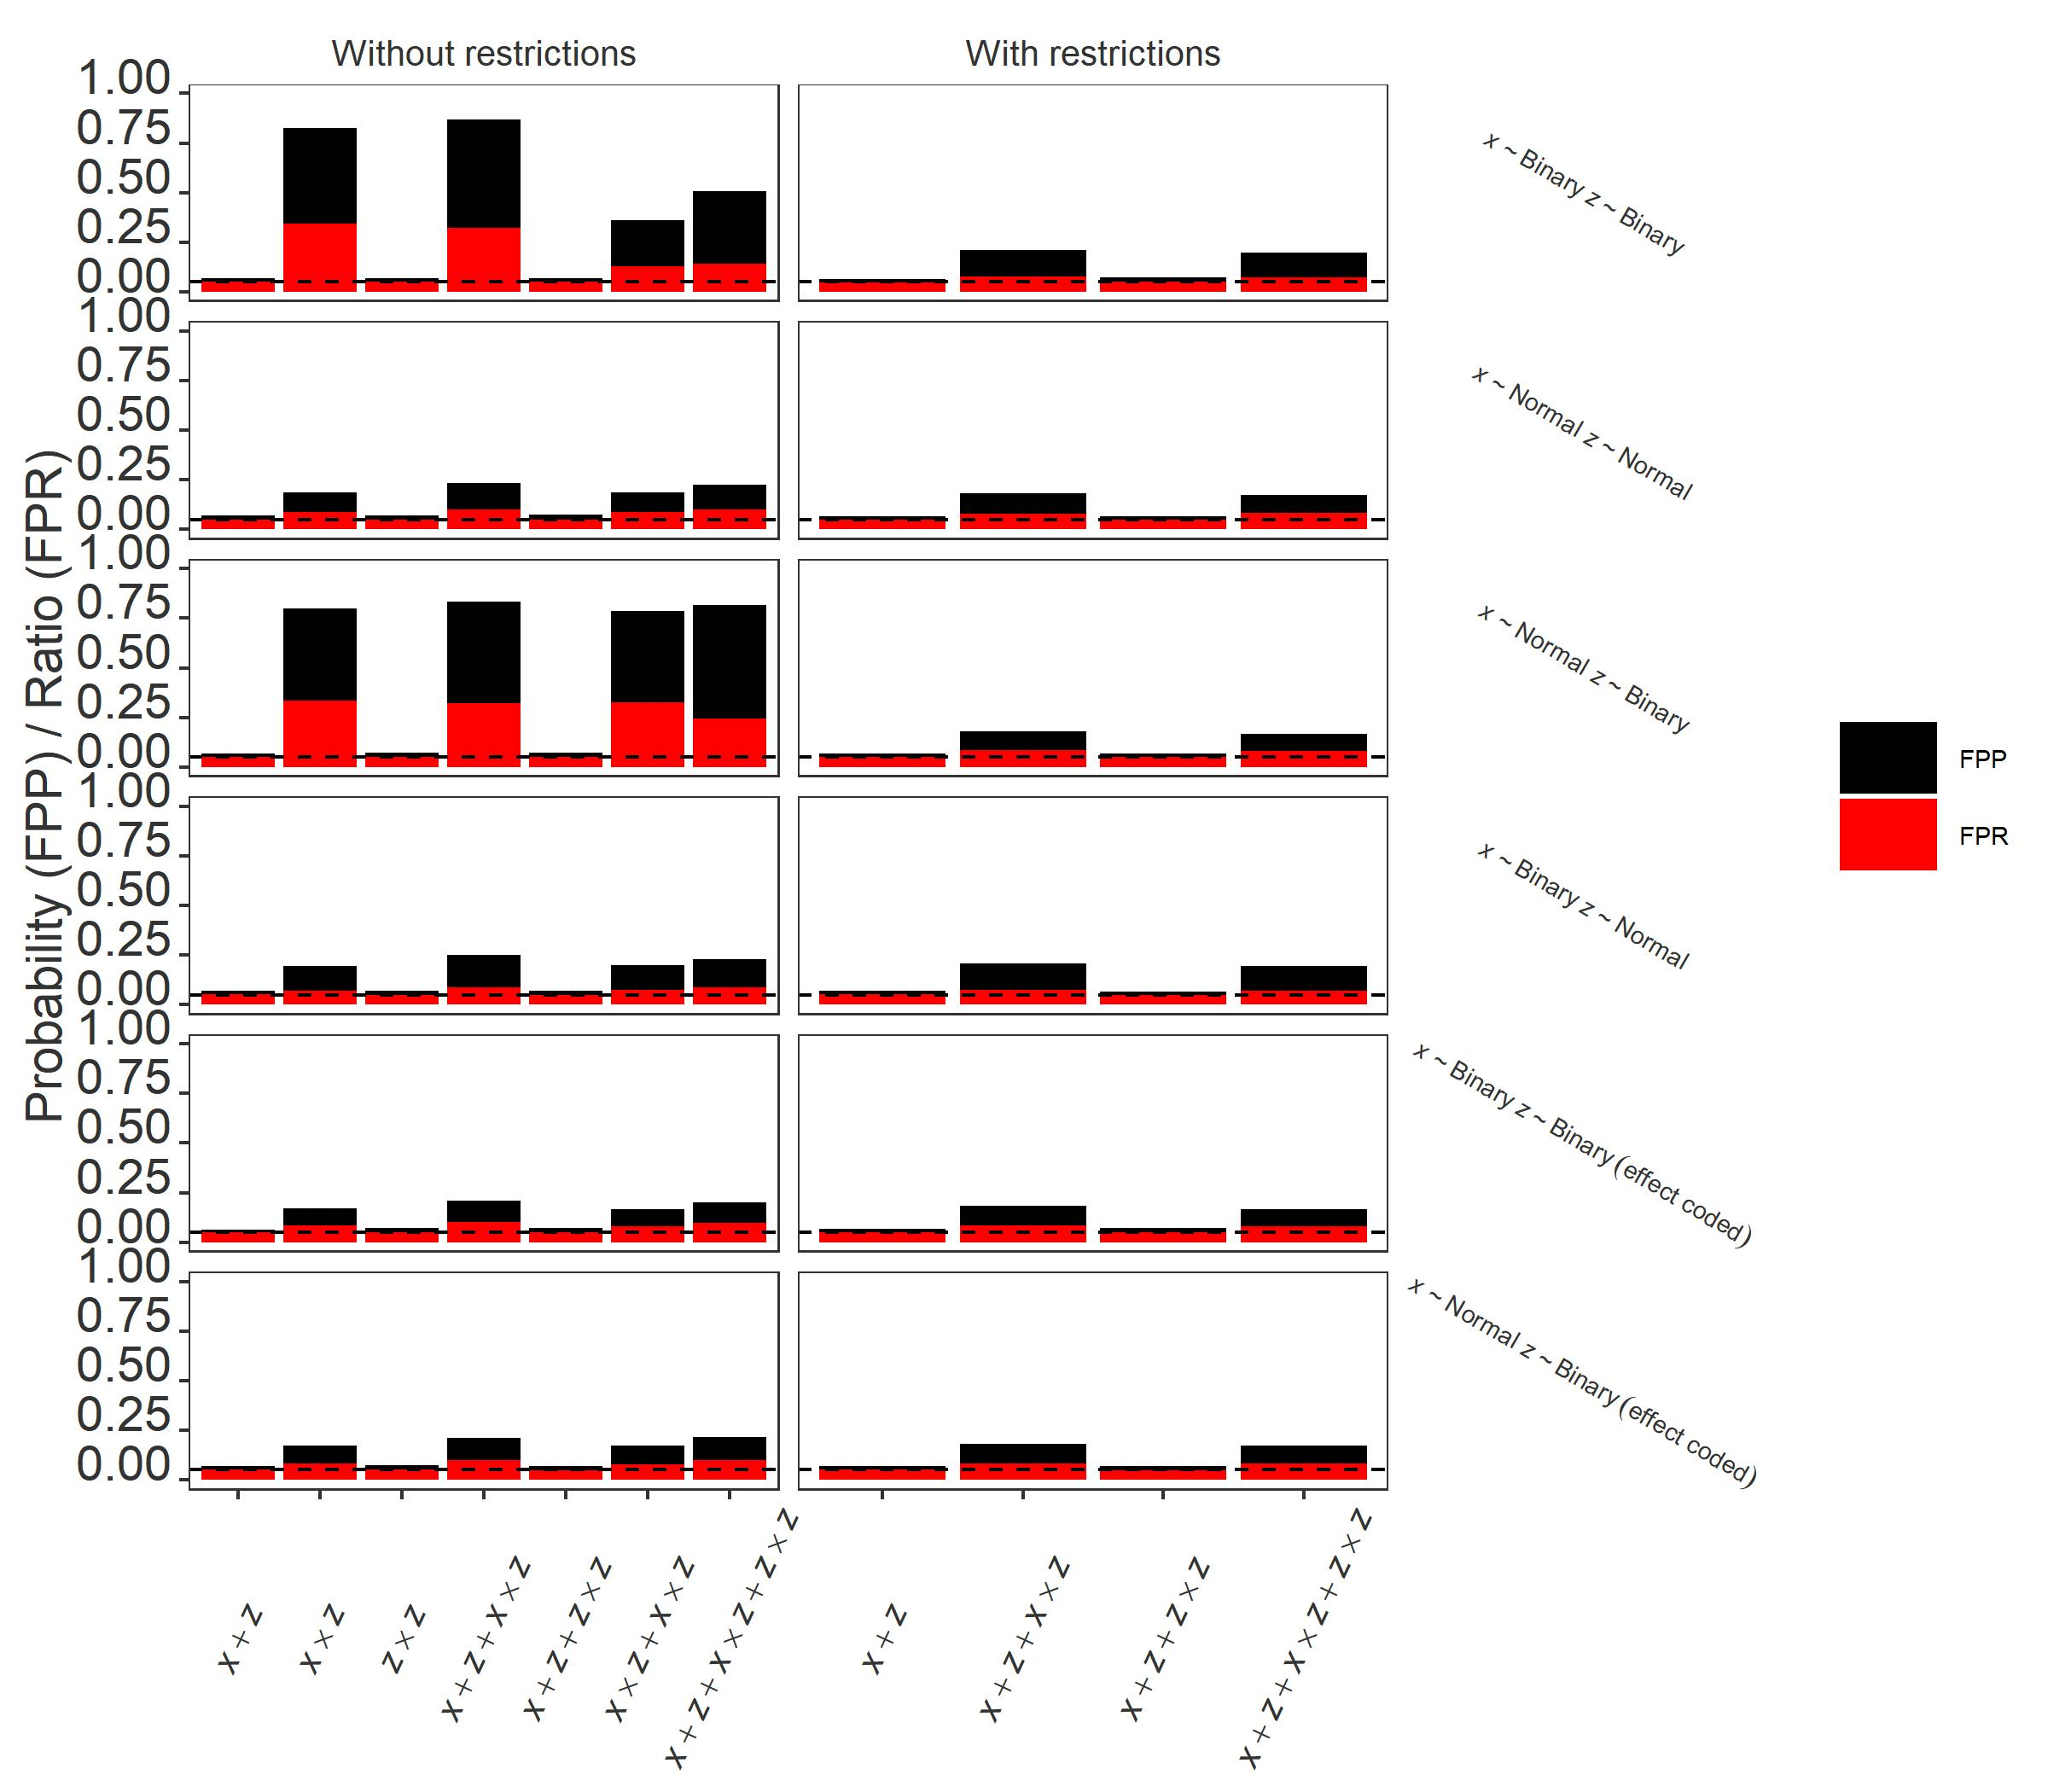
\includegraphics[scale=0.95]{R/Analysis/Result/Figures/Figure1ASI.jpeg}
\centering
\caption{The probability of the false positive probability and false positive ratio given different model sets, the presence of main effects when having interactions (i.e., With restrictions for interactions or No restrictions for interactions) and different distributions of the variable of interest and covariates. Sample size was set to 200, a correlation between the dependent variable and covariates was \textit{r}=0.2 and we used two covariates. The false positive probability is shown in black and the false positive ratio in red. Here binary variables are both shown when it is dummy coded (Co=Binary) but also effects coded (Co=Binary Effect).}
\label{fig:mainfigure}
\end{figure}


\begin{figure}[hbt!]
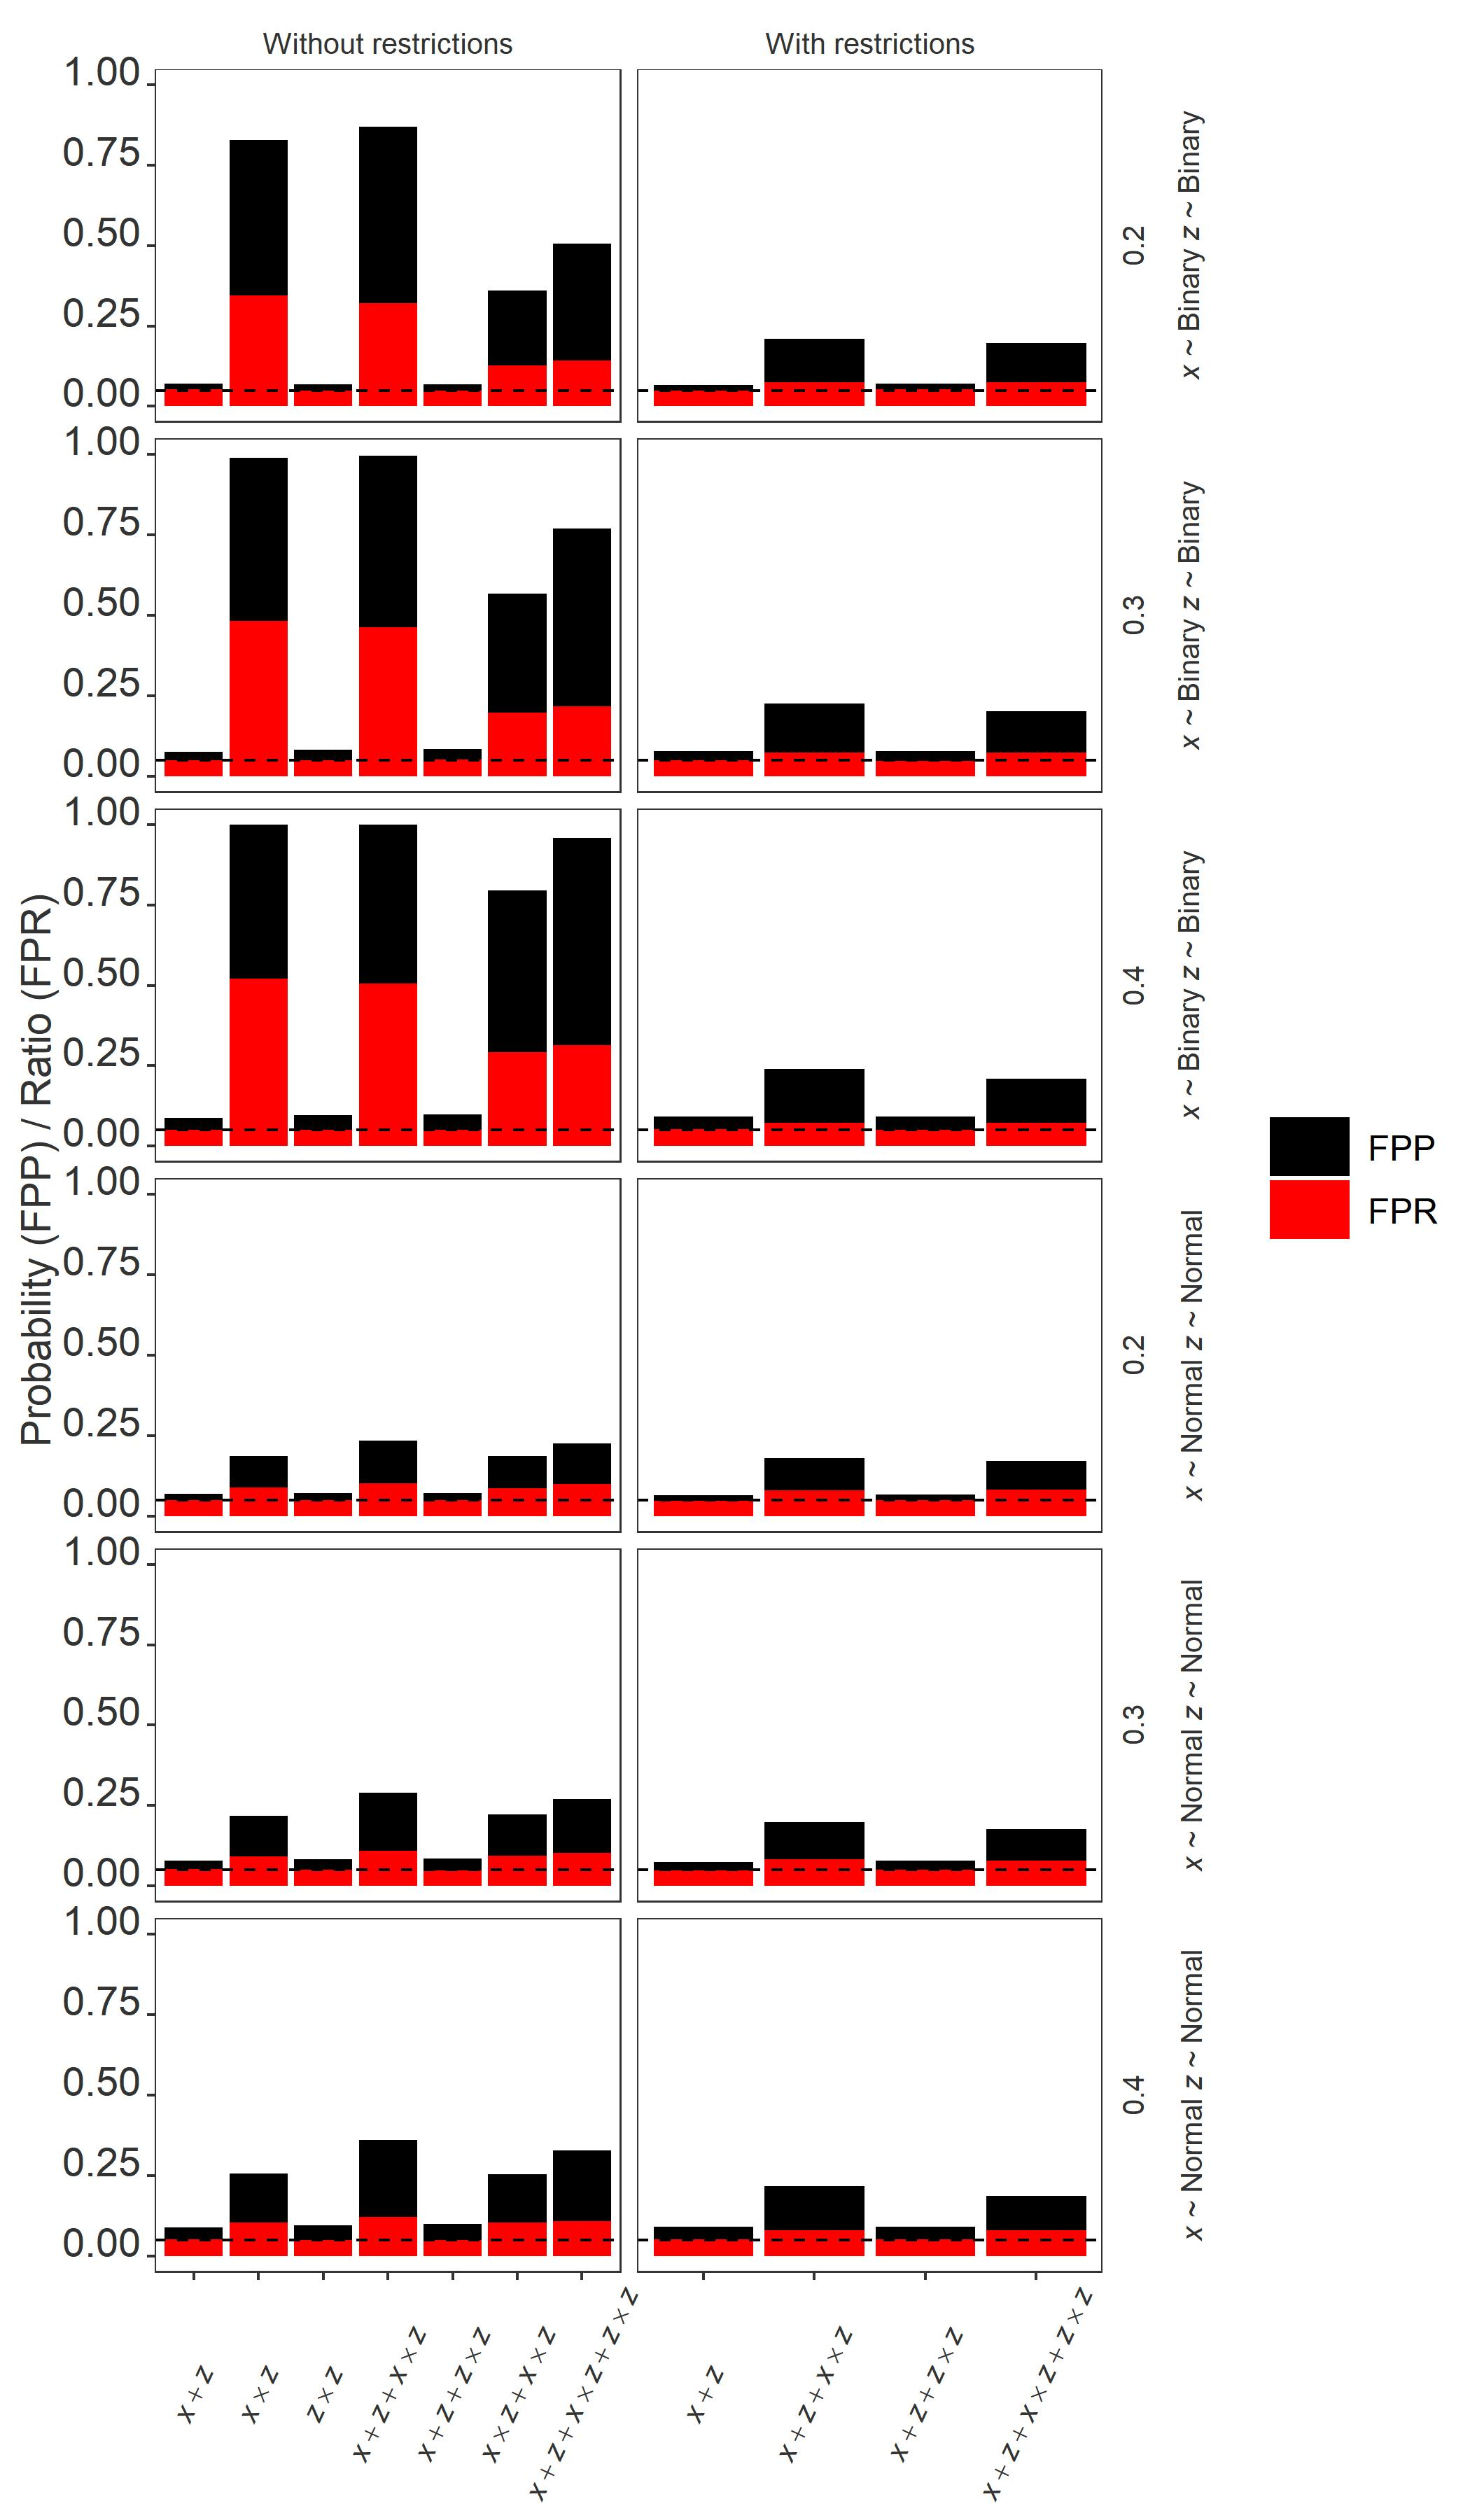
\includegraphics[scale=0.7]{R/Analysis/Result/Figures/Figure2SI.jpeg}
\centering
\caption{False positive probability and false positive for different levels of correlation between the dependent variable and the covariates ranging from r=0.2 to r=0.4. Black denotes the false positive probability and red denotes the false positive ratio. The description of the figure is otherwise the same as for Figure S1.}
\label{fig:mainfigure}
\end{figure}


\begin{figure}[hbt!]
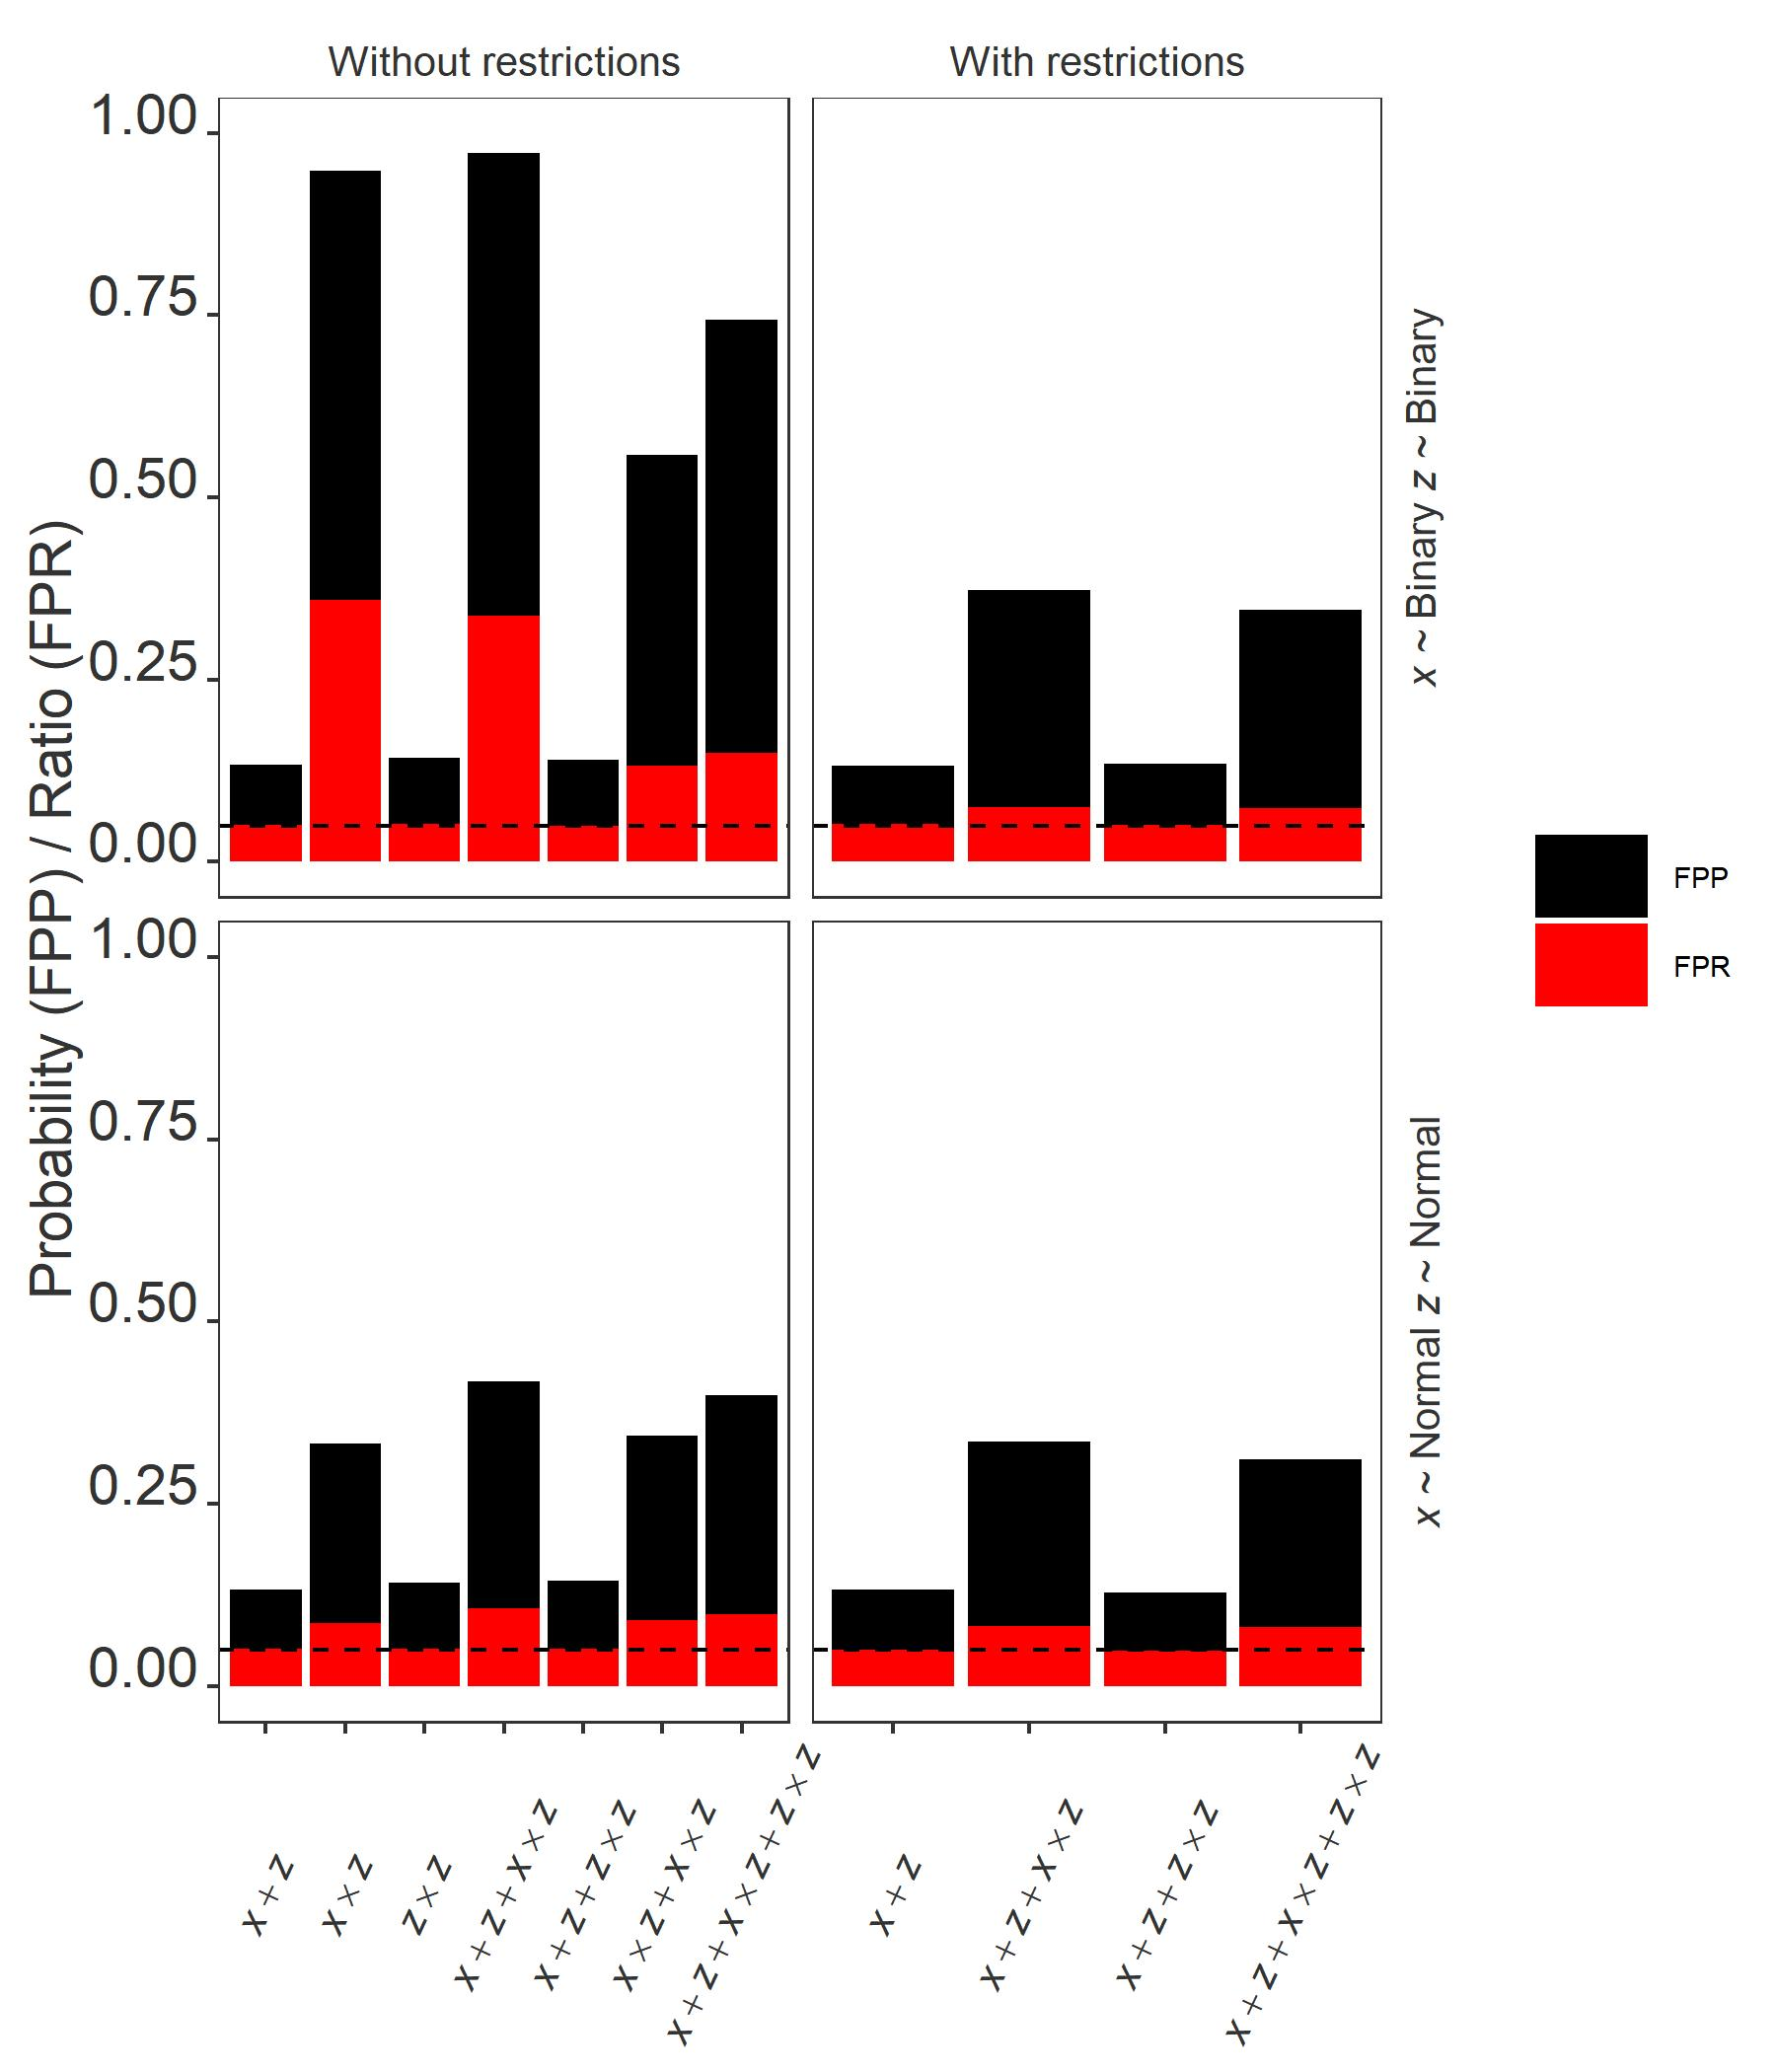
\includegraphics{R/Analysis/Result/Figures/Figure3SI.jpeg}
\centering
\caption{False positive probability and false positive ratio when using two dependent variables and the average of the two (meaning three dependent variables in total). The correlation between the dependent variables is set to r=0.5 with the correlation between the dependent variables and covariates still at r=0.2. Black denotes the the false positive probability and red denotes the false positive ratio. The description of the figure is otherwise the same as for Figure S1.}
\label{fig:mainfigure}
\end{figure}


\begin{figure}[hbt!]
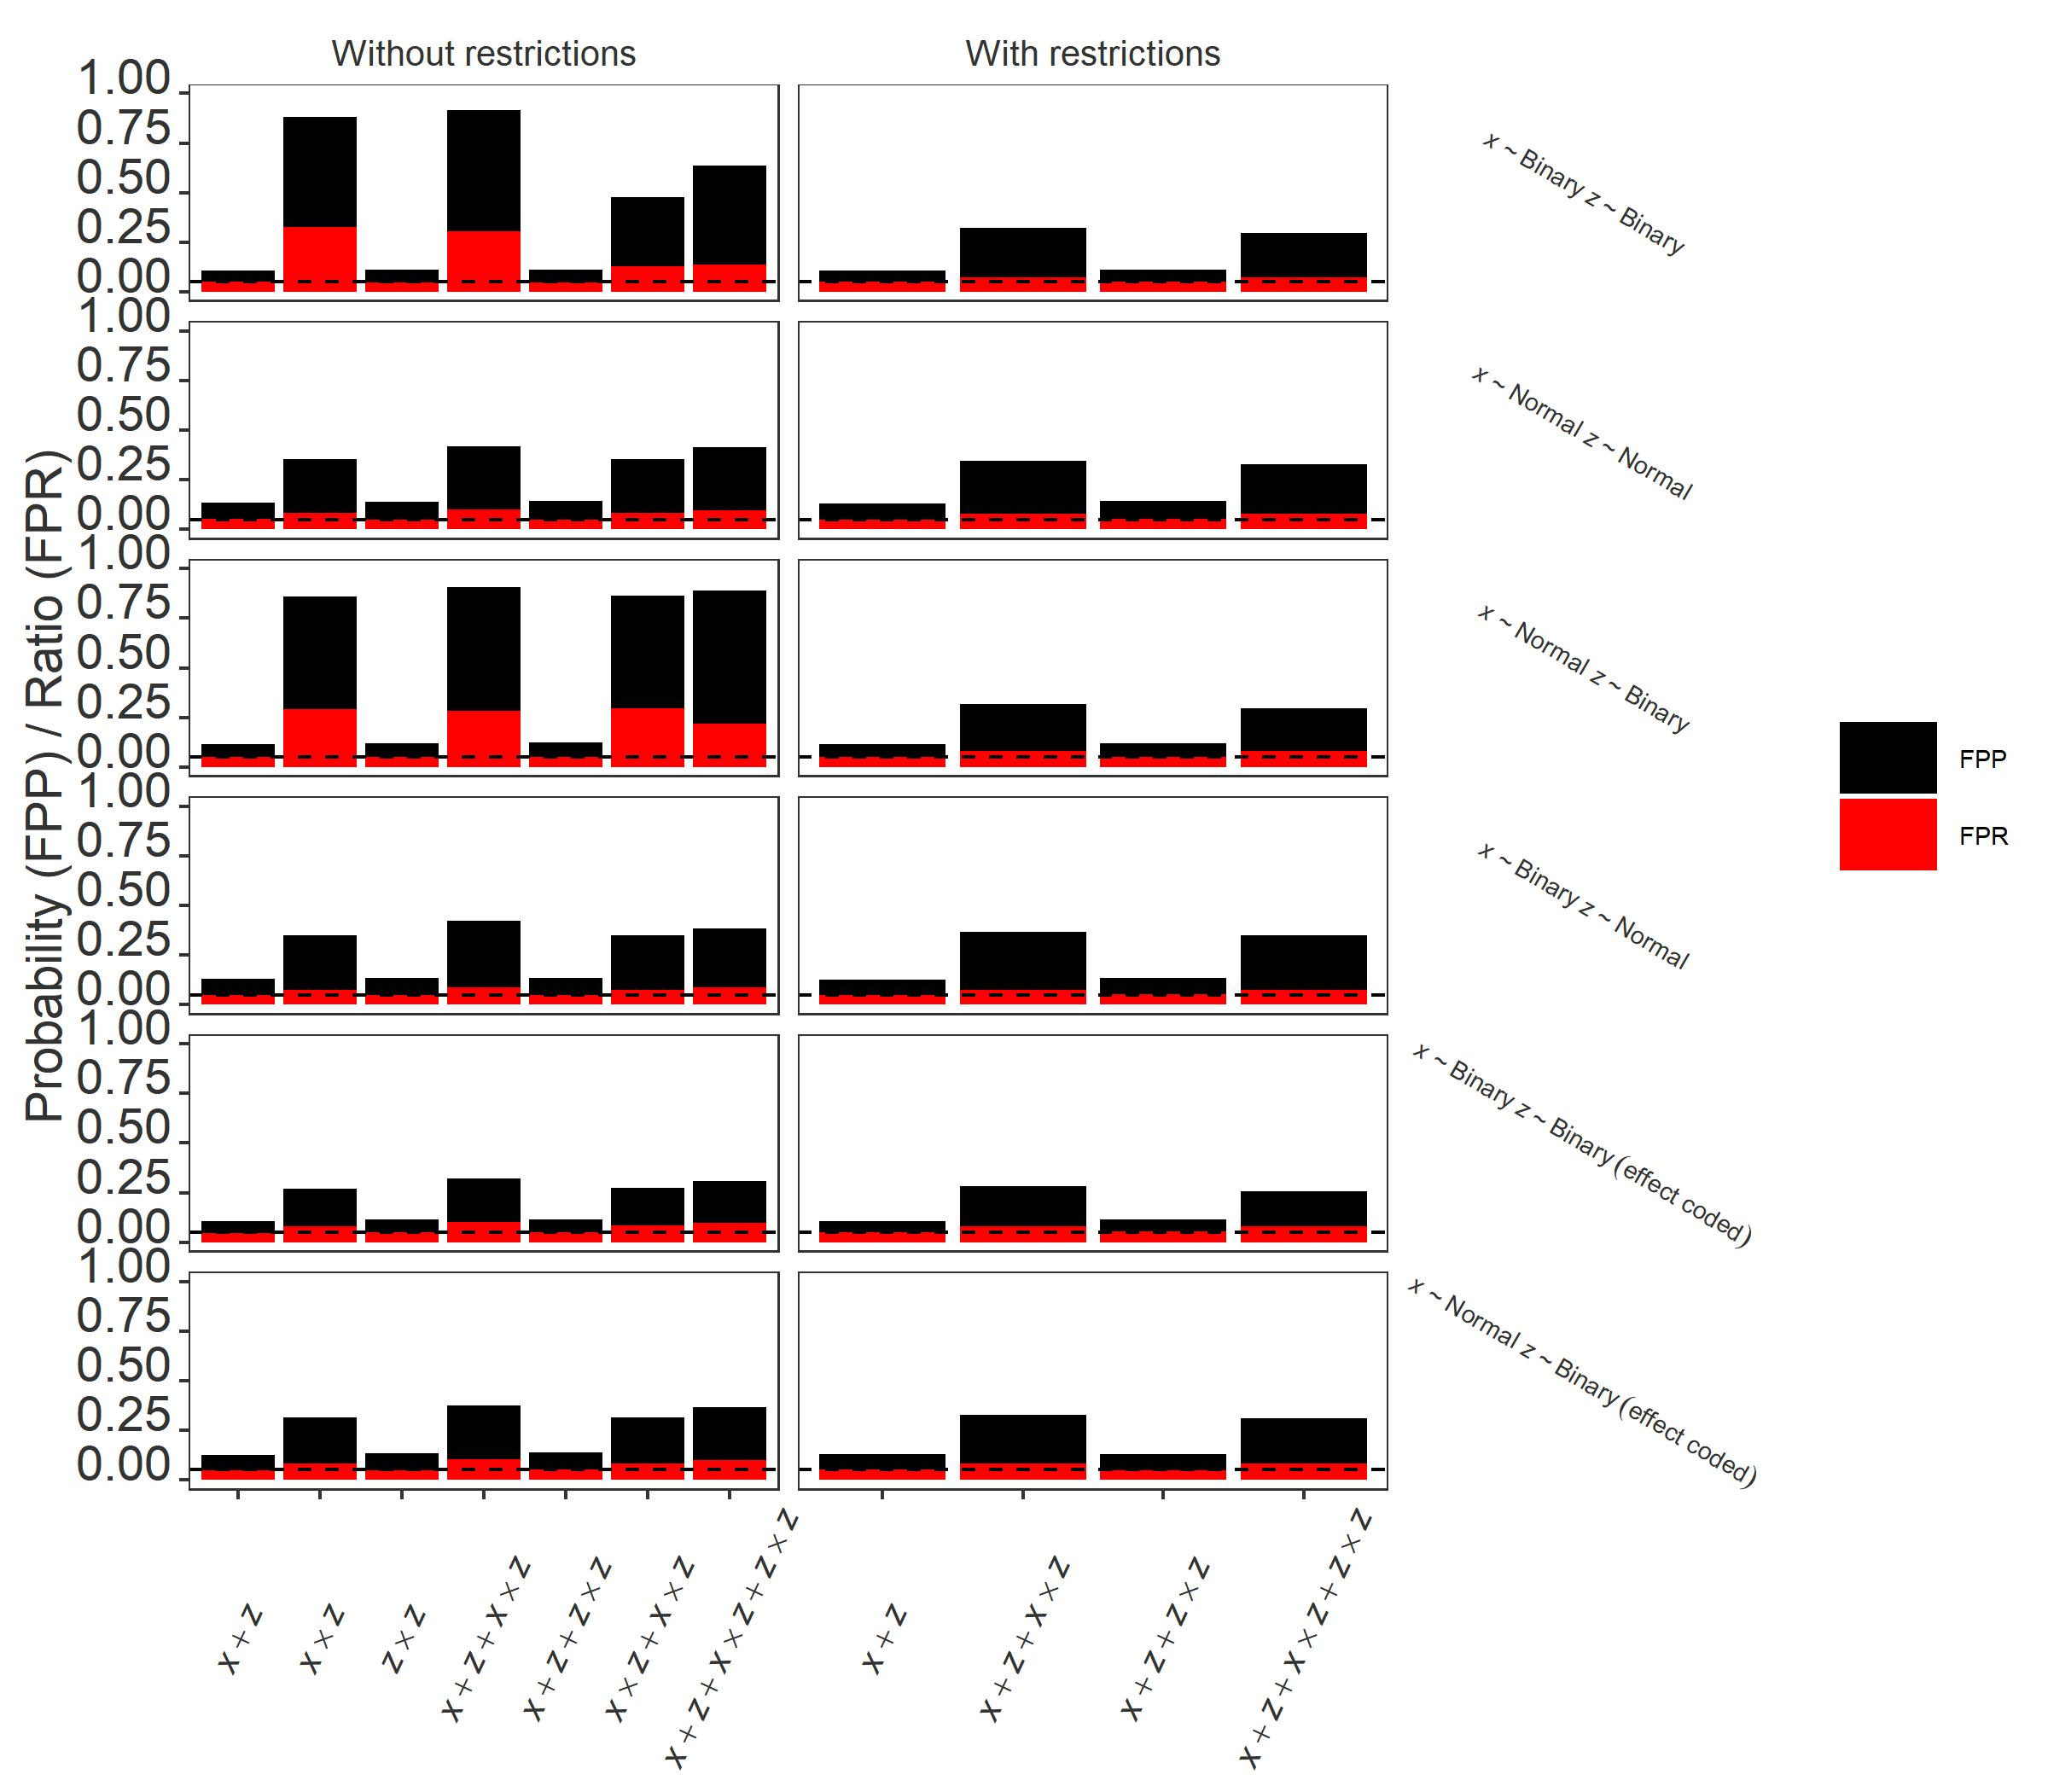
\includegraphics[scale=0.95]{R/Analysis/Result/Figures/Figure1BSI.jpeg}
\centering
\caption{False positive probability and false positive ratio when using multiple outlier criteria. Black denotes the the false positive probability and red denotes the false positive ratio. The description of the figure is otherwise the same as for Figure S1.
}
\label{fig:mainfigure}
\end{figure}

\begin{figure}[hbt!]
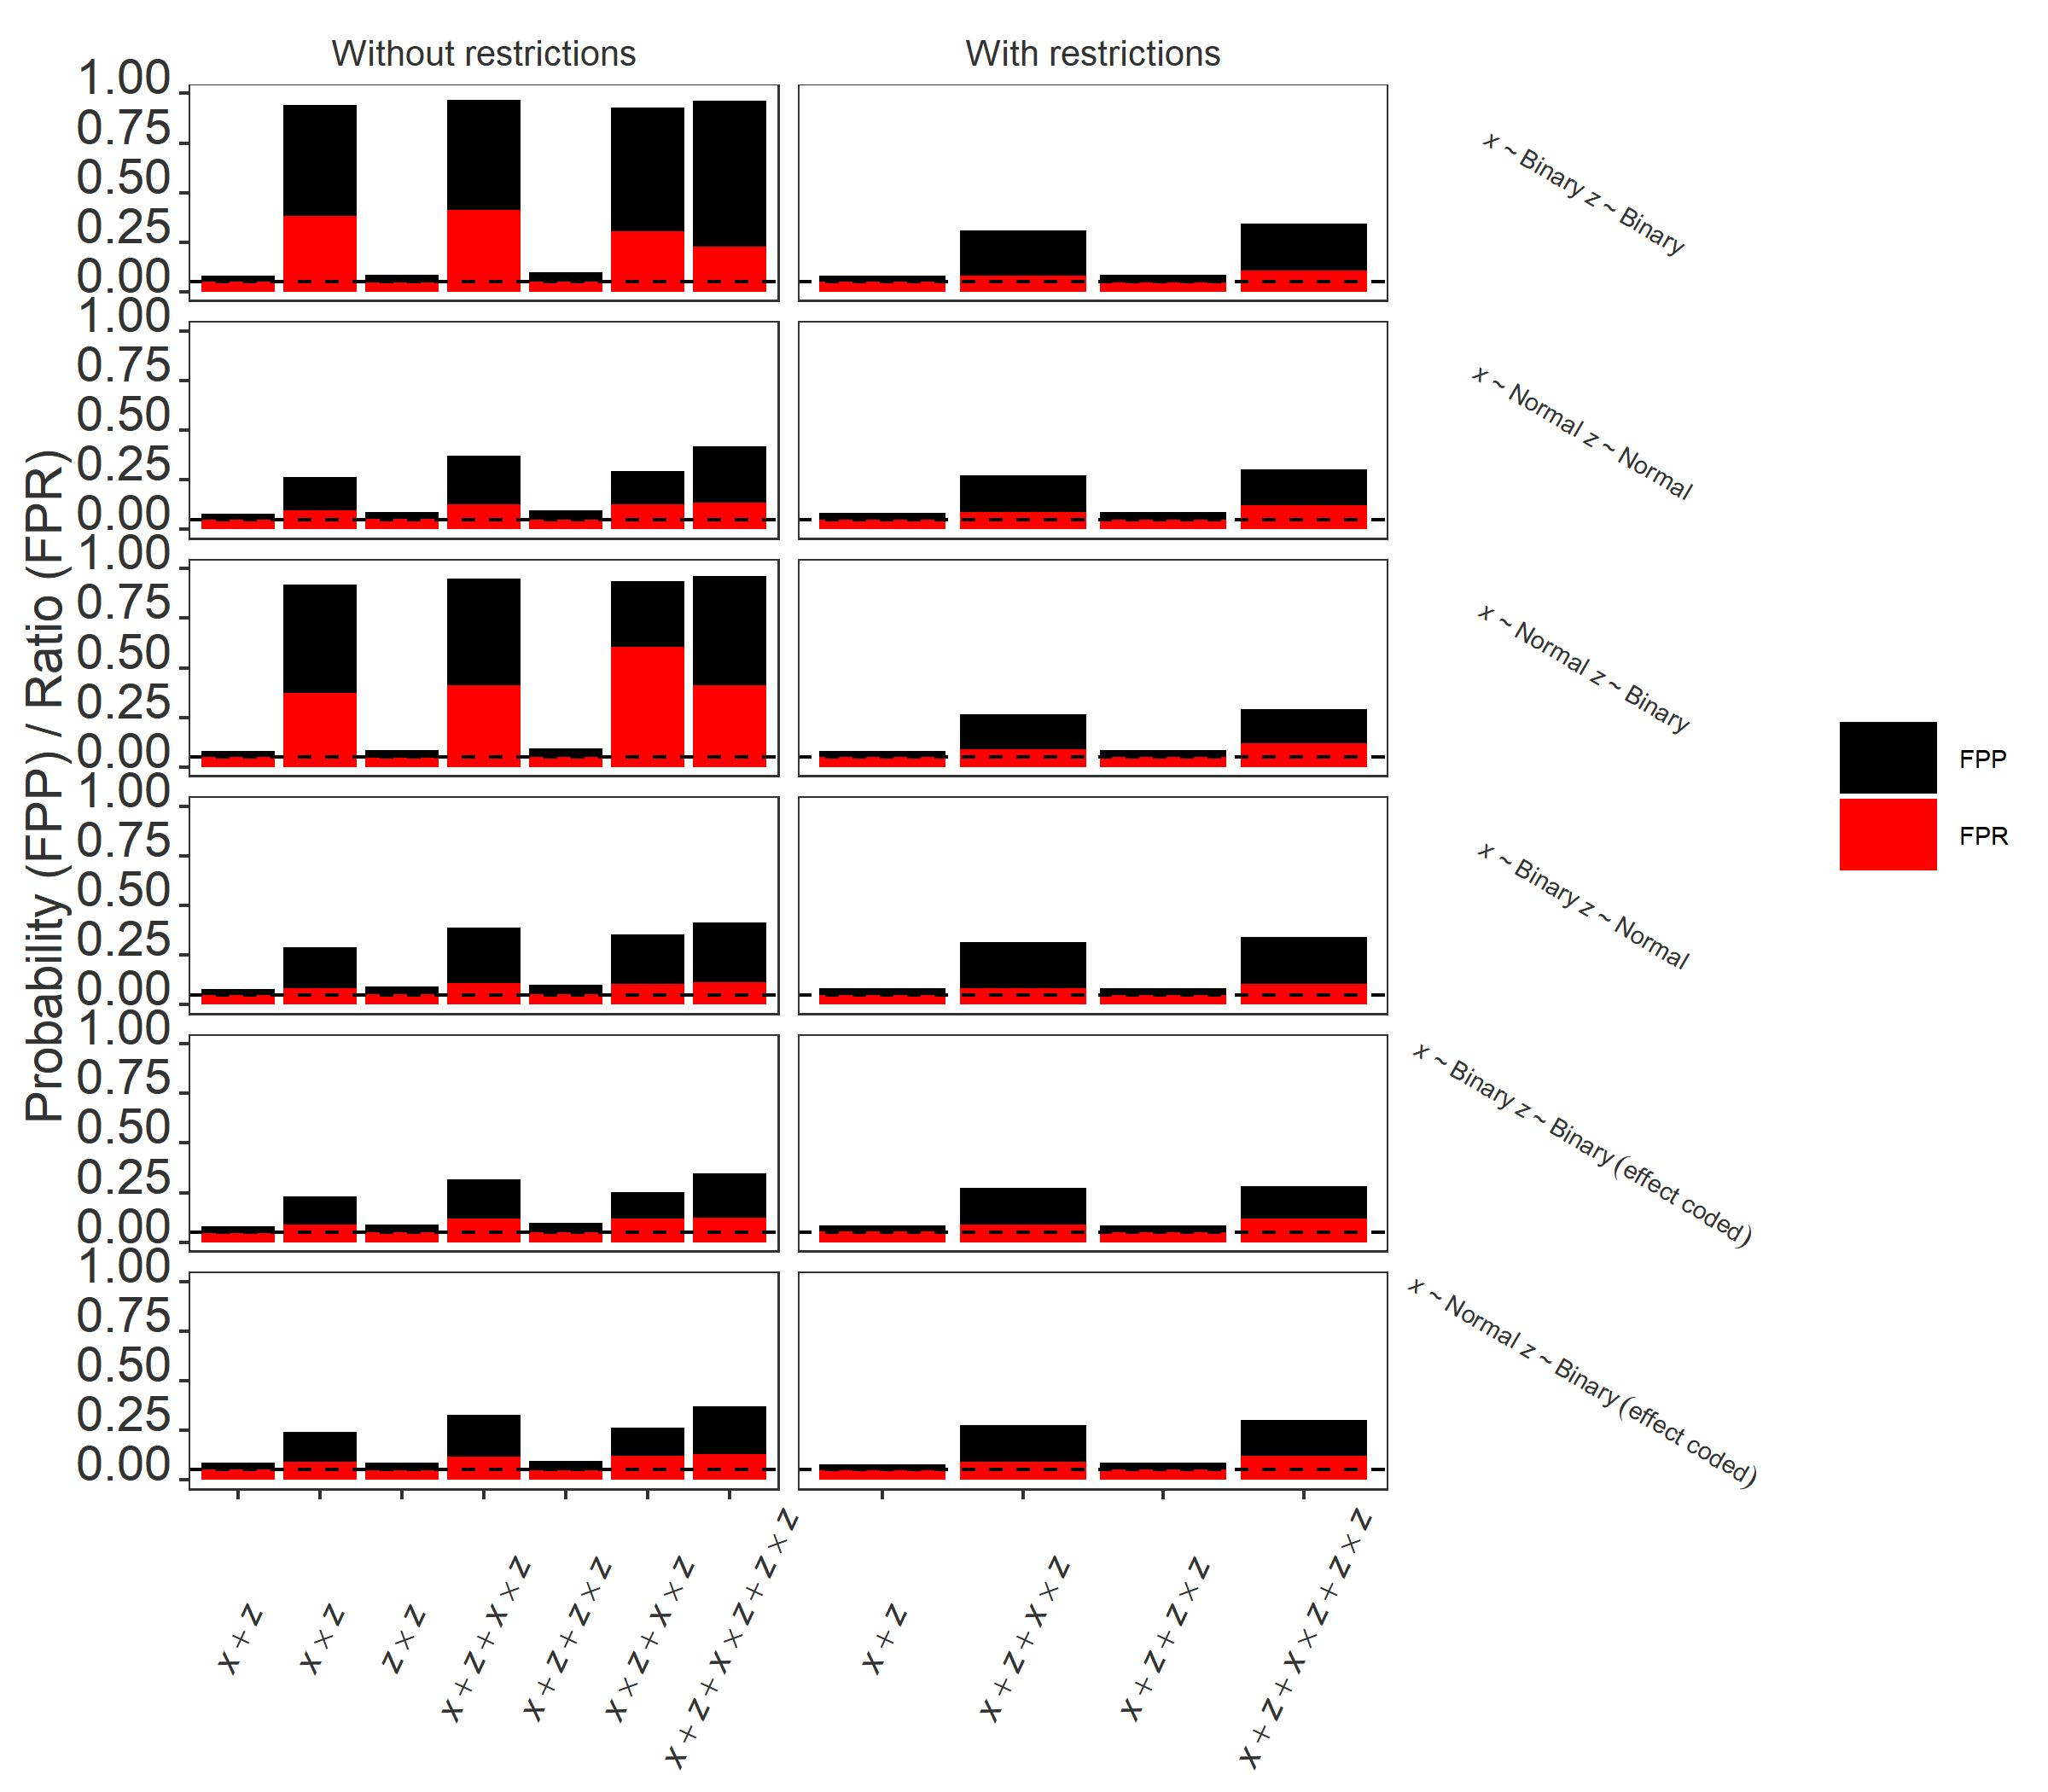
\includegraphics[scale=0.95]{R/Analysis/Result/Figures/Figure1CSI.jpeg}
\centering
\caption{False positive probability and false positive ratio when using three covariates instead of two as in the base line model. Black denotes the the false positive probability and red denotes the false positive ratio. The description of the figure is otherwise the same as for Figure S1.
}
\label{fig:mainfigure}
\end{figure}

\begin{landscape}
\begin{figure}[hbt!]
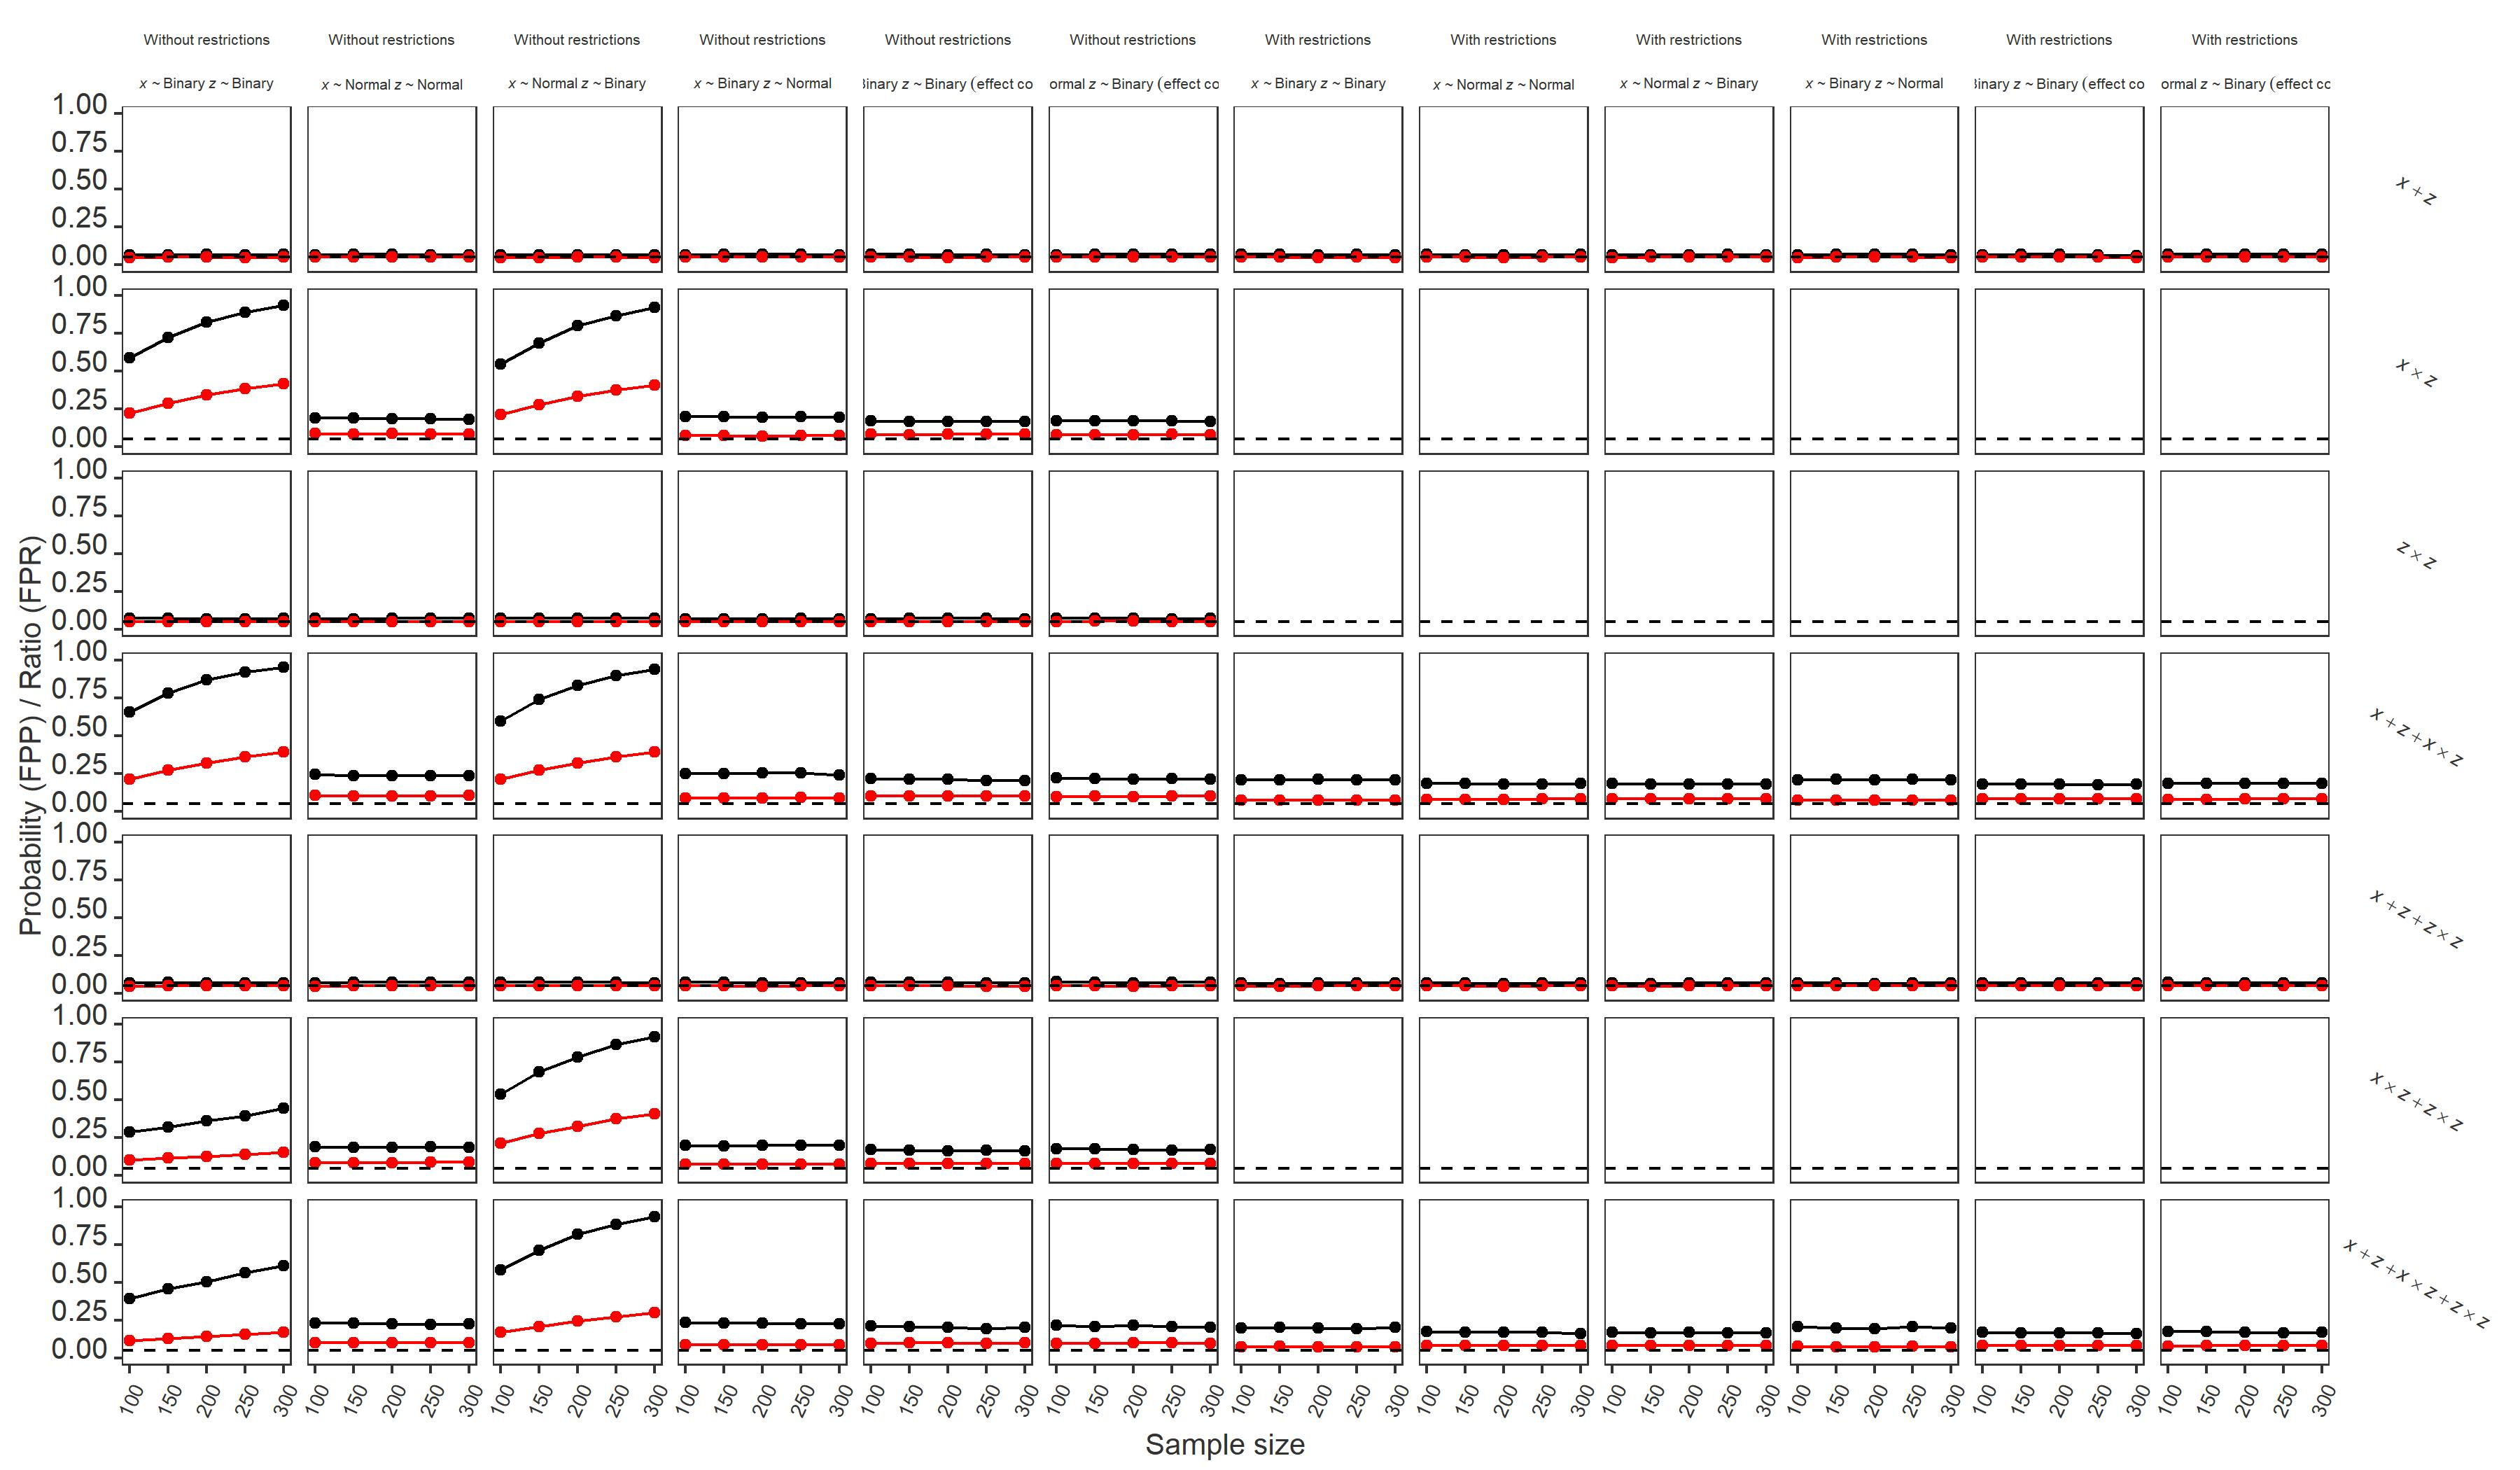
\includegraphics[scale=0.75]{R/Analysis/Result/Figures/Figure1DSI.jpeg}
\centering
\caption{Effect of increasing sample size for each model set and all combinations of data distributions (i.e., binary and normal). Black denotes the false positive probability and red denotes the false positive ratio. The description of the figure is otherwise the same as for Figure S1.}
\label{fig:mainfigure}
\end{figure}
\end{landscape}

\clearpage
\subsection{Results when using Bonferroni correction}

In this section, we present the same analyses but with Bonferroni correction applied. 

Table S13 shows the FPP and FPR for the full model sets under different conditions when there is used Bonferroni correction. Here there is no split between each model set.This lowers the FPR to the expected 5\% but there is still an issue when not including main effects and having binomial variables. 


% latex table generated in R 4.0.0 by xtable 1.8-4 package
% Wed Jan 27 11:47:03 2021
\begin{longtable}{llrr}
\caption{False positive probability (FPP) and false positive ratio (FPR) when looking at all the models possible when the sample size is 200, no outlier criteria is being used and having two covariates. When restrictions on interactions are on main effects should always be present when there is interactions, this is not the case when restrictions on interactions is off.} \\ 
  \hline
Restrictions on interactions & Type & FPP & FPR \\ 
  \hline
Without & Normal & 0.16 & 0.05 \\ 
  Without & Binomial & 0.75 & 0.16 \\ 
  With & Normal & 0.12 & 0.05 \\ 
  With & Binomial & 0.14 & 0.04 \\ 
   \hline
\hline
\end{longtable}


\begin{figure}[hbt!]
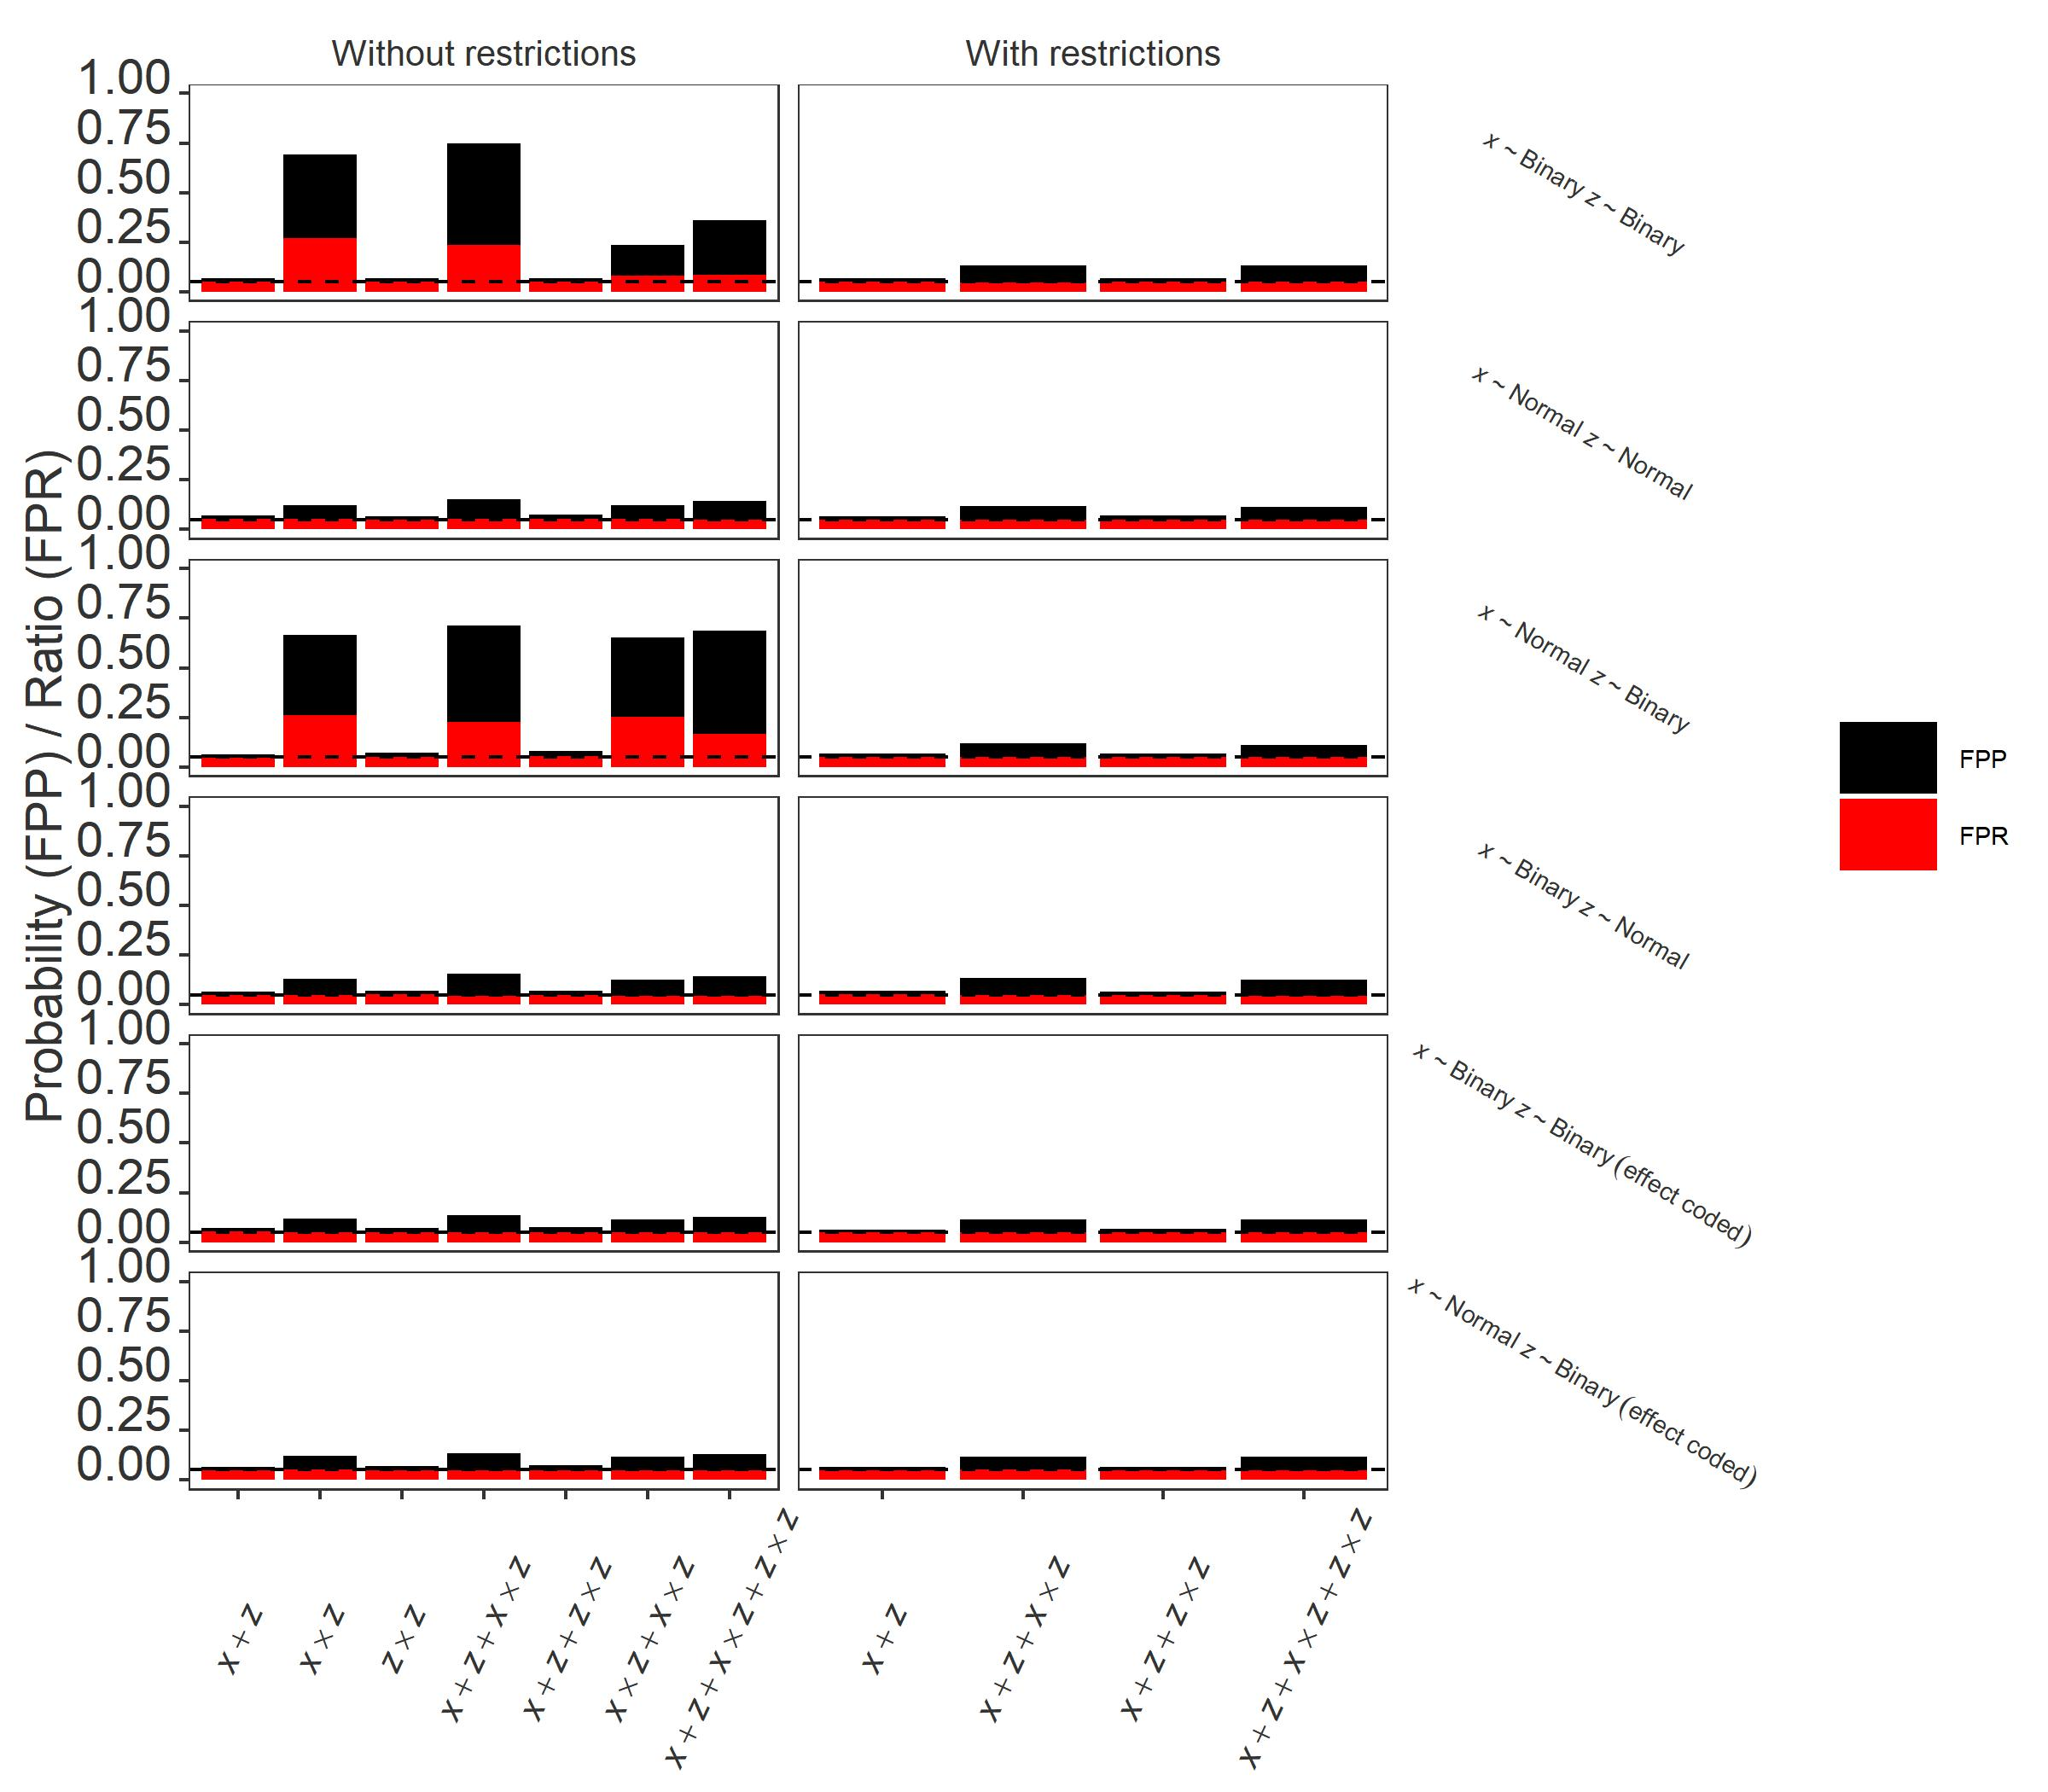
\includegraphics[scale=0.95]{R/Analysis/Result/Figures/Figure1ASIBon.jpeg}
\centering
\caption{The description of this figure is the same as for Figure S1 with the only difference being that we applied Bonferroni correction. This figure therefore shows the probability of the false positive probability and false positive ratio given different model sets, the presence of main effects when having interactions (i.e., With restrictions for interactions or No restrictions for interactions) and different distributions of the variable of interest and covariates. Sample size was set to 200, a correlation between the dependent variable and covariates was \textit{r}=0.2 and we used two covariates. The false positive probability is shown in black and the false positive ratio in red. Here binary variables are both shown when it is dummy coded (Co=Binary) but also effects coded (Co=Binary Effect).}
\label{fig:mainfigure}
\end{figure}


\begin{figure}[hbt!]
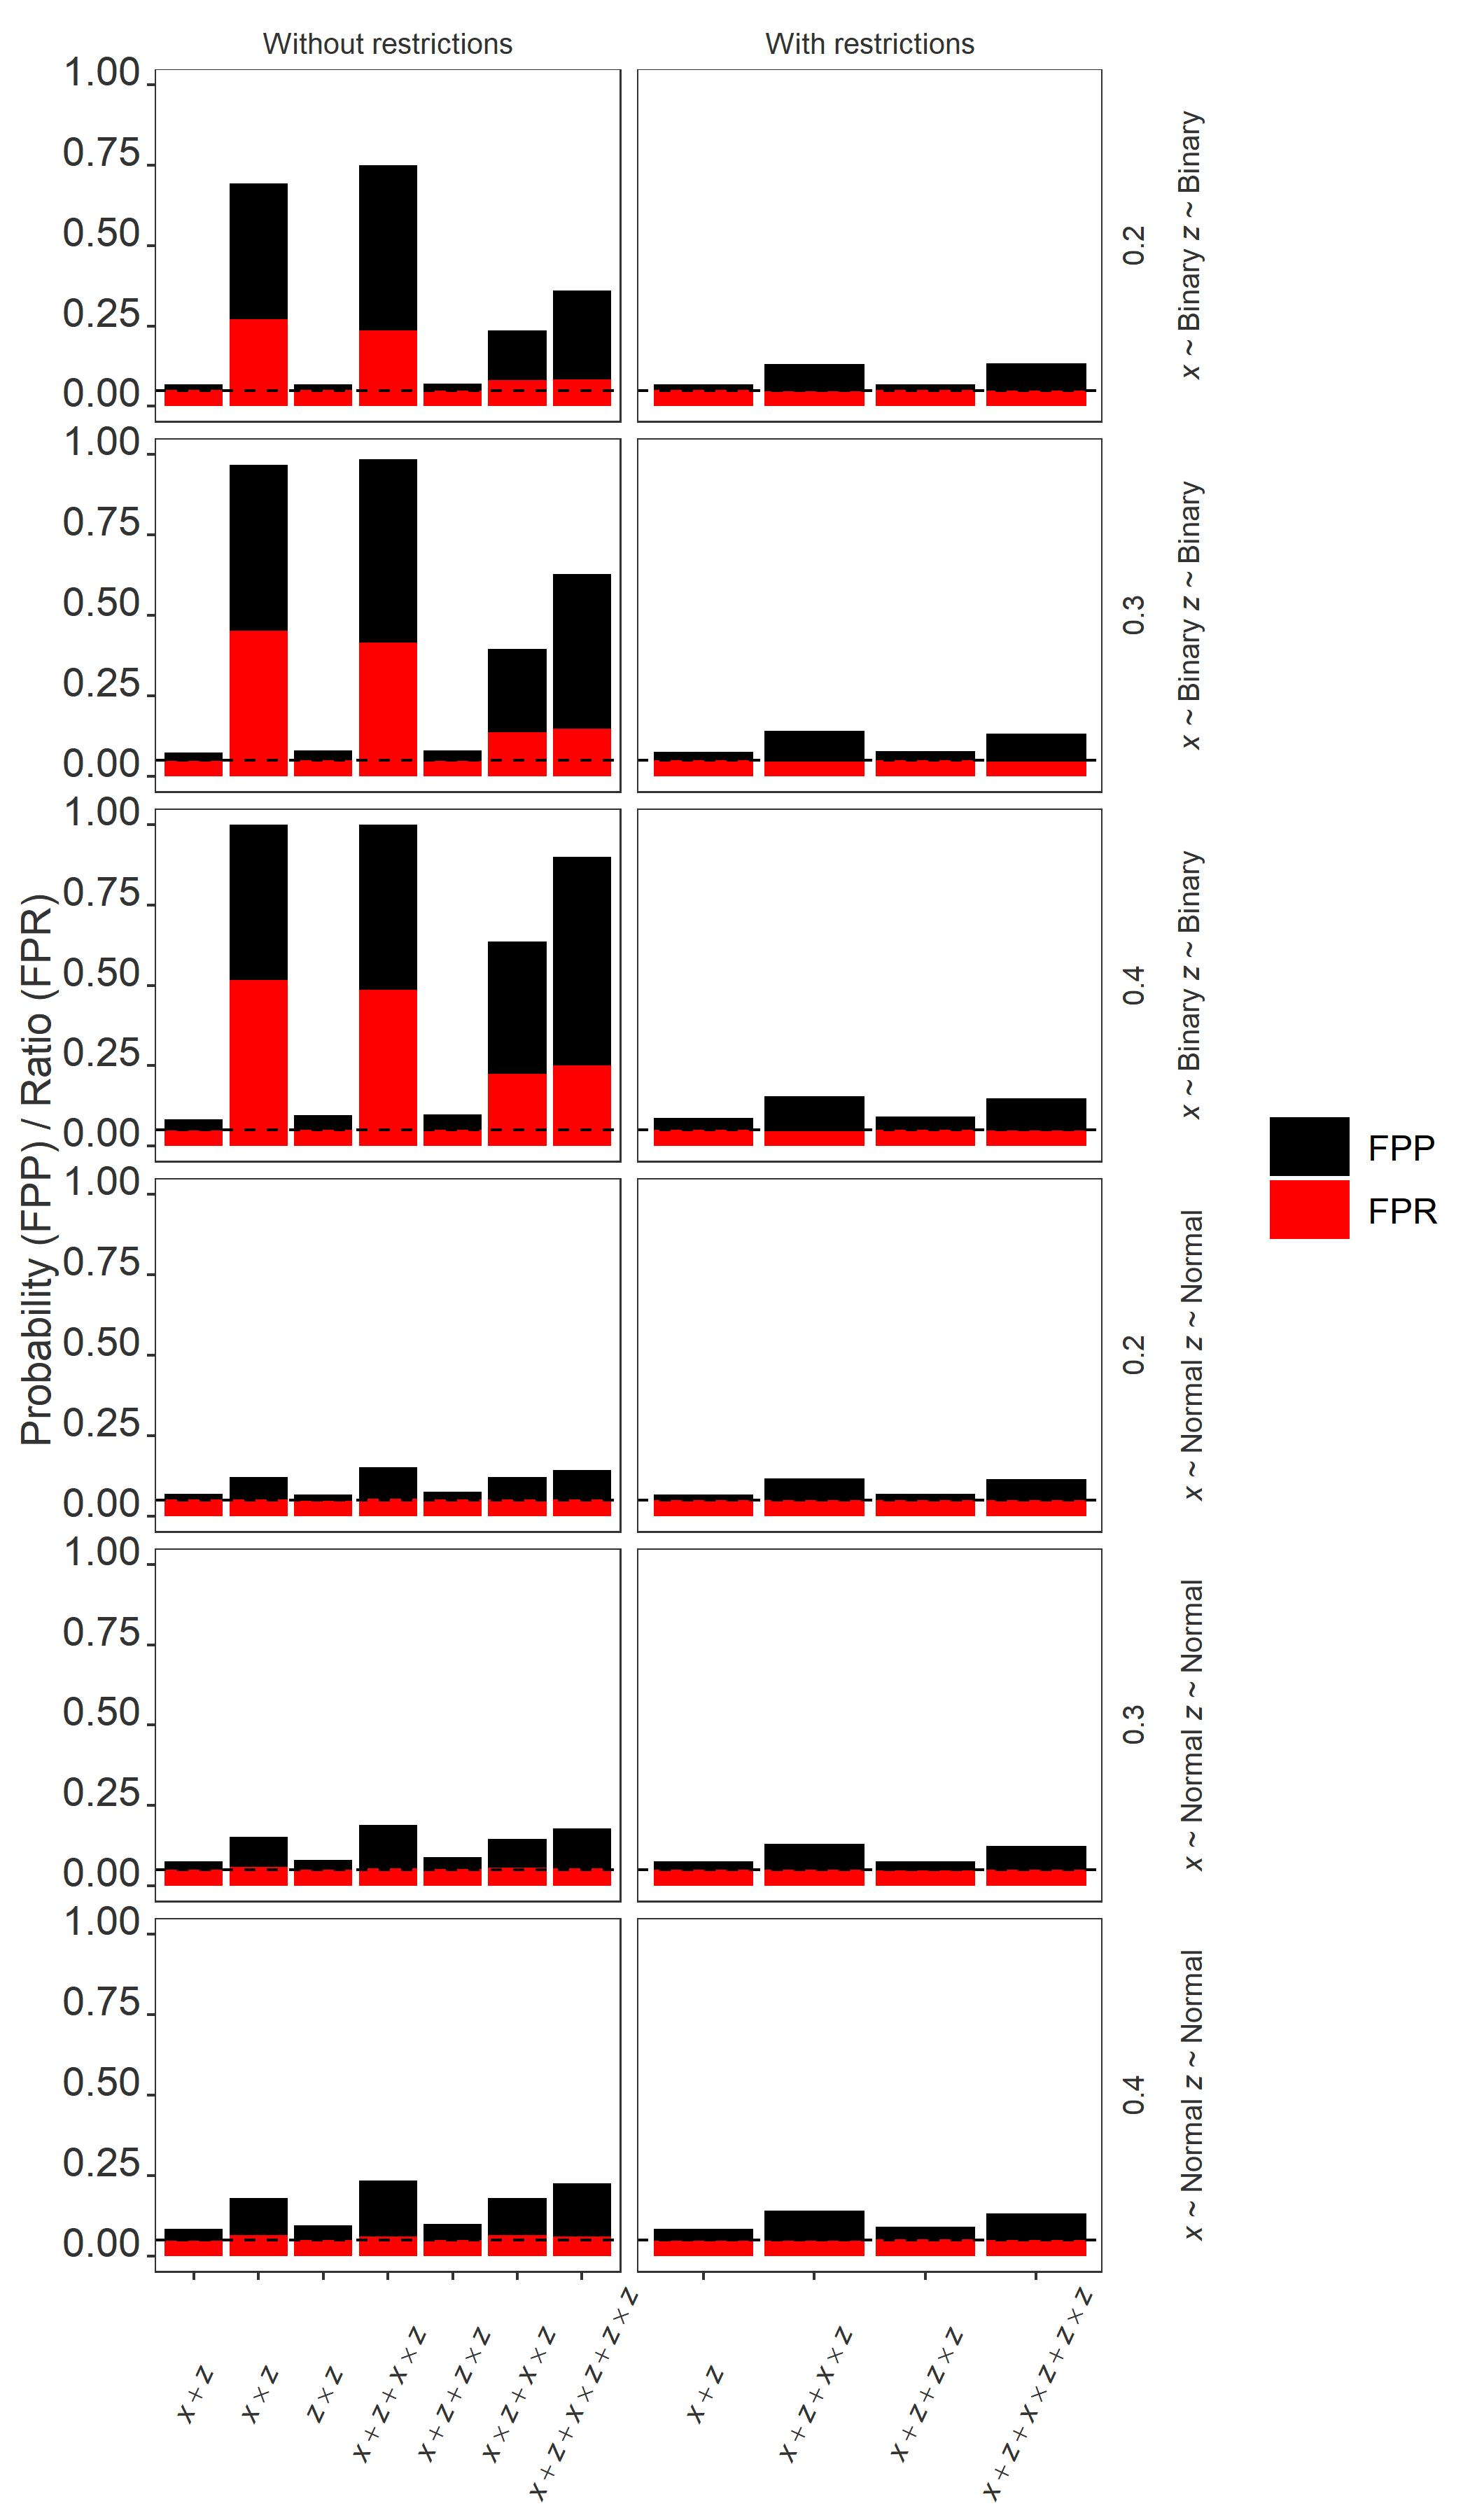
\includegraphics[scale=0.7]{R/Analysis/Result/Figures/Figure2SIBon.jpeg}
\centering
\caption{False positive probability and false positive for different levels of correlation between the dependent variable and the covariates ranging from r=0.2 to r=0.4. Black denotes the false positive probability and red denotes the false positive ratio. The description of the figure is otherwise the same as for Figure S7.}
\label{fig:mainfigure}
\end{figure}


\begin{figure}[hbt!]
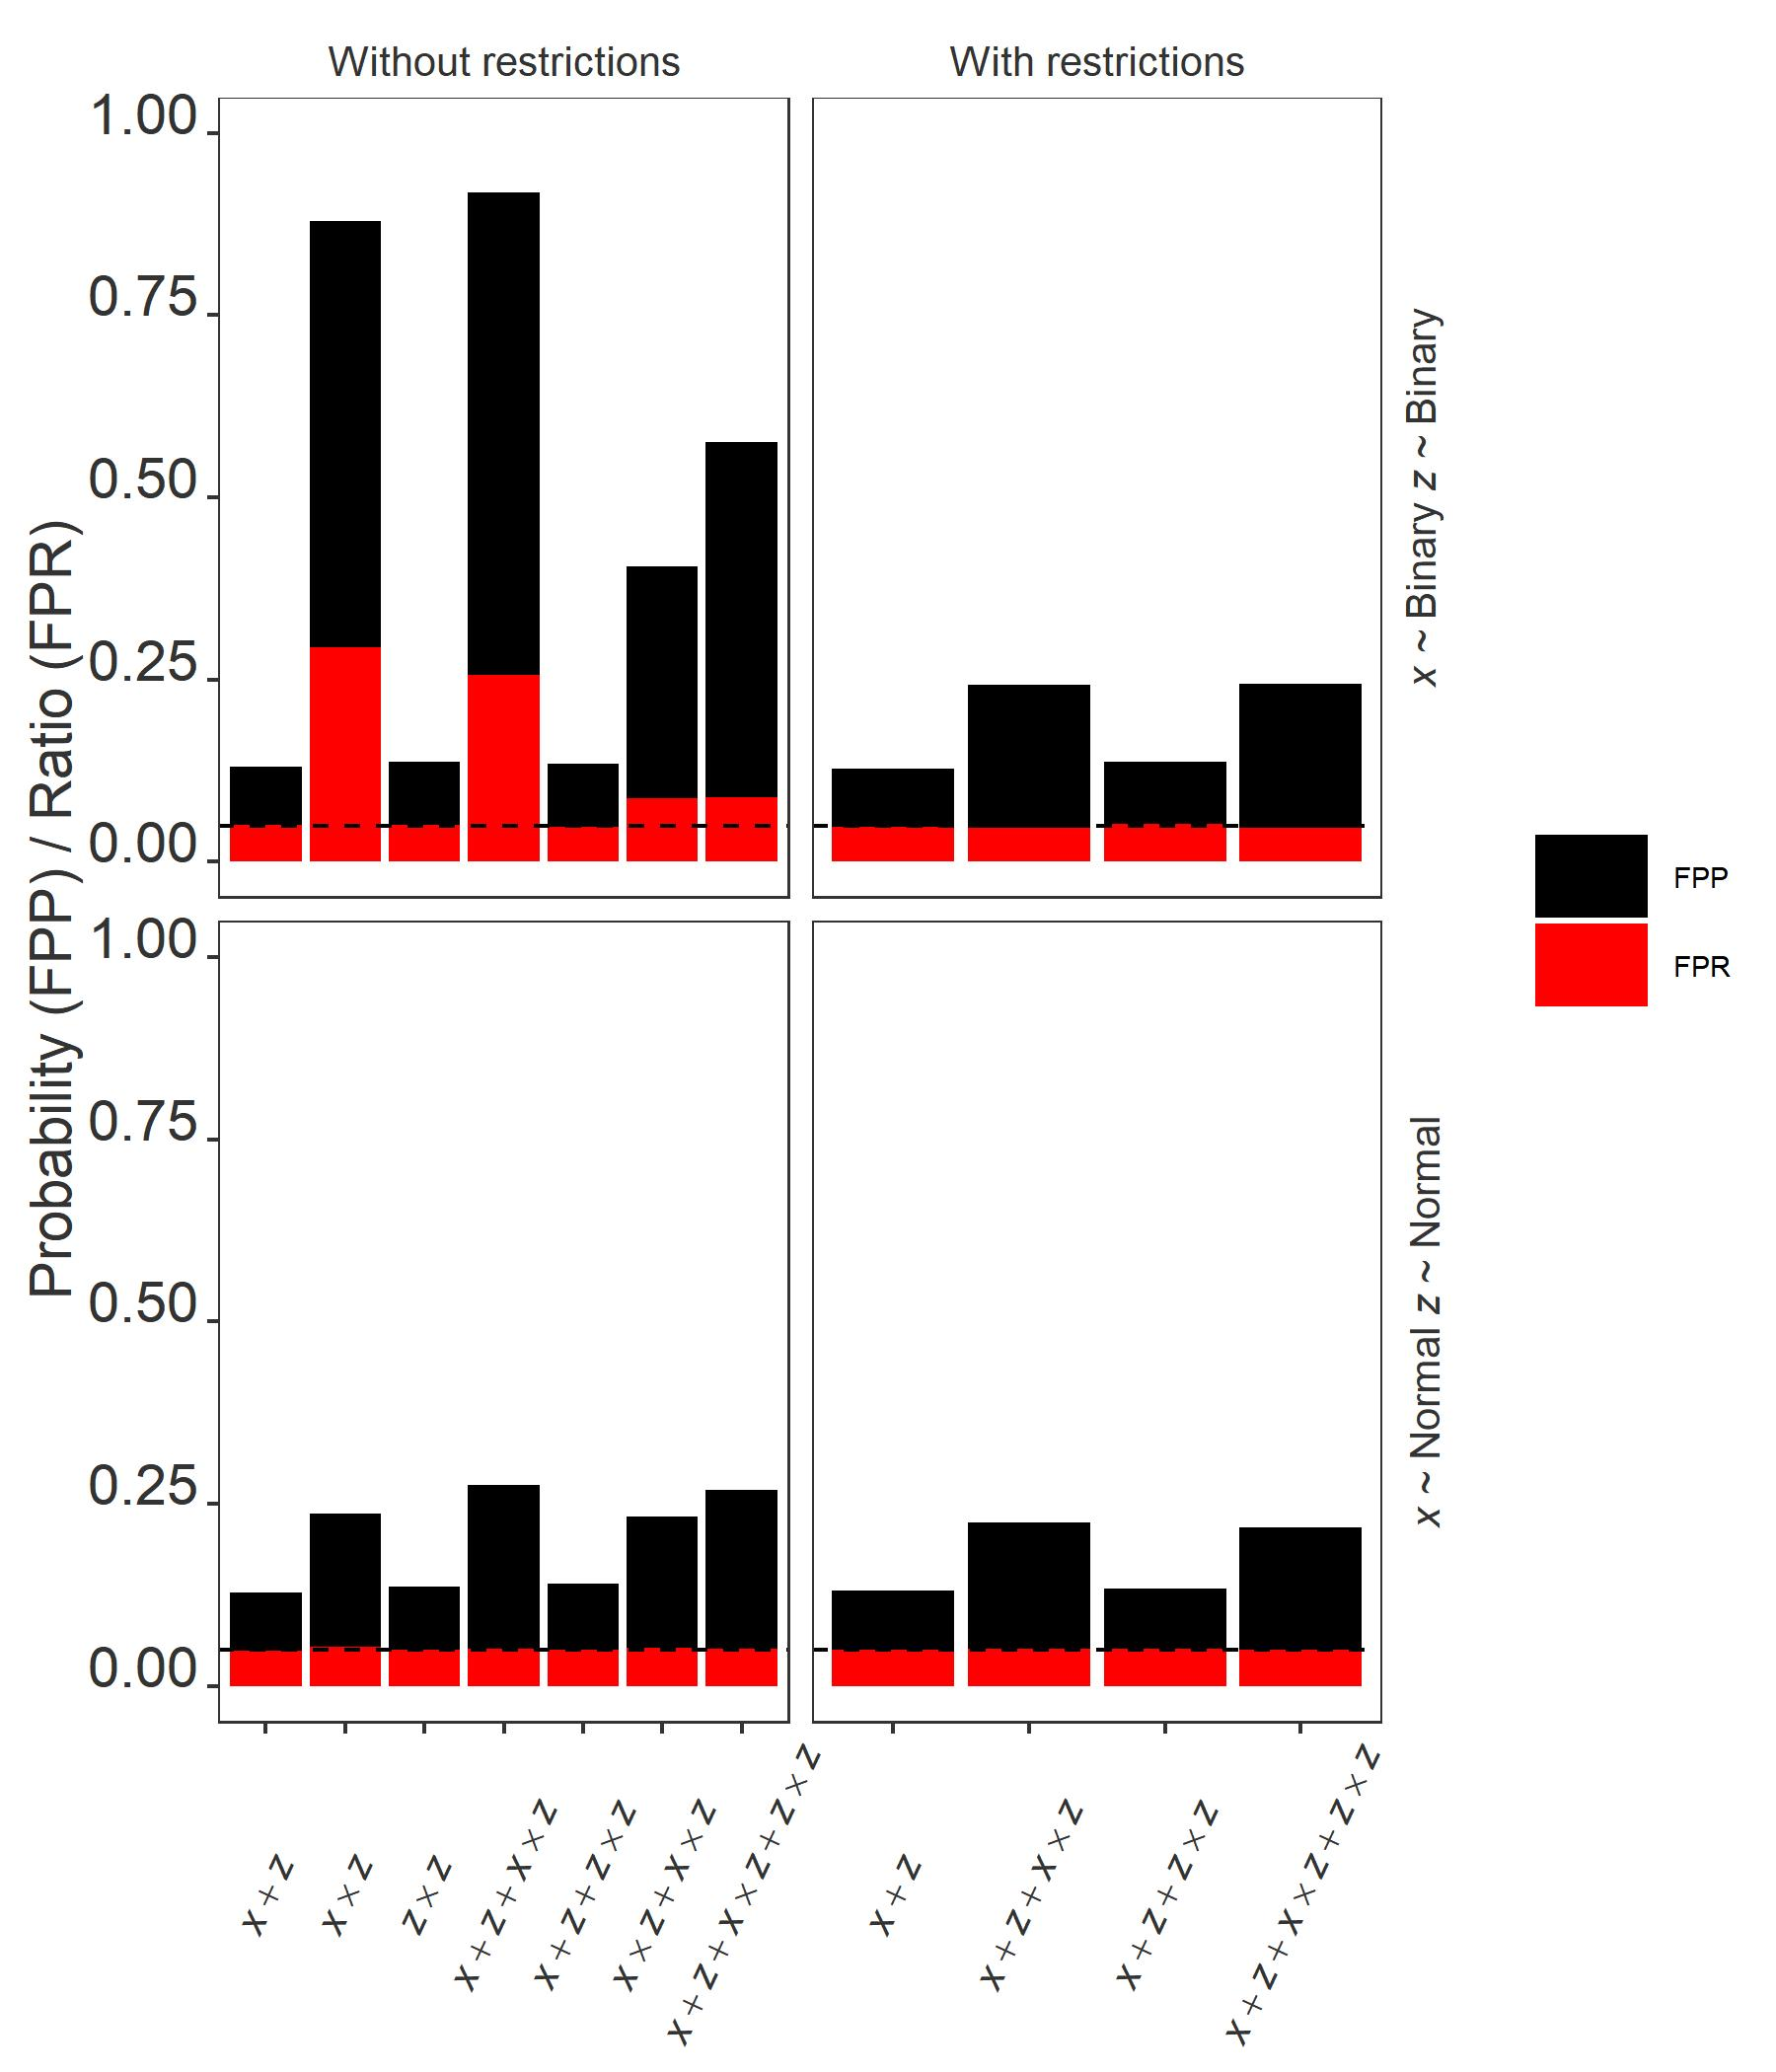
\includegraphics{R/Analysis/Result/Figures/Figure3SIBon.jpeg}
\centering
\caption{False positive probability and false positive ratio when using two dependent variables and the average of the two (meaning three dependent variables in total). The correlation between the dependent variables is set to r=0.5 with the correlation between the dependent variables and covariates still at r=0.2. Black denotes the the false positive probability and red denotes the false positive ratio. The description of the figure is otherwise the same as for Figure S7.}
\label{fig:mainfigure}
\end{figure}


\begin{figure}[hbt!]
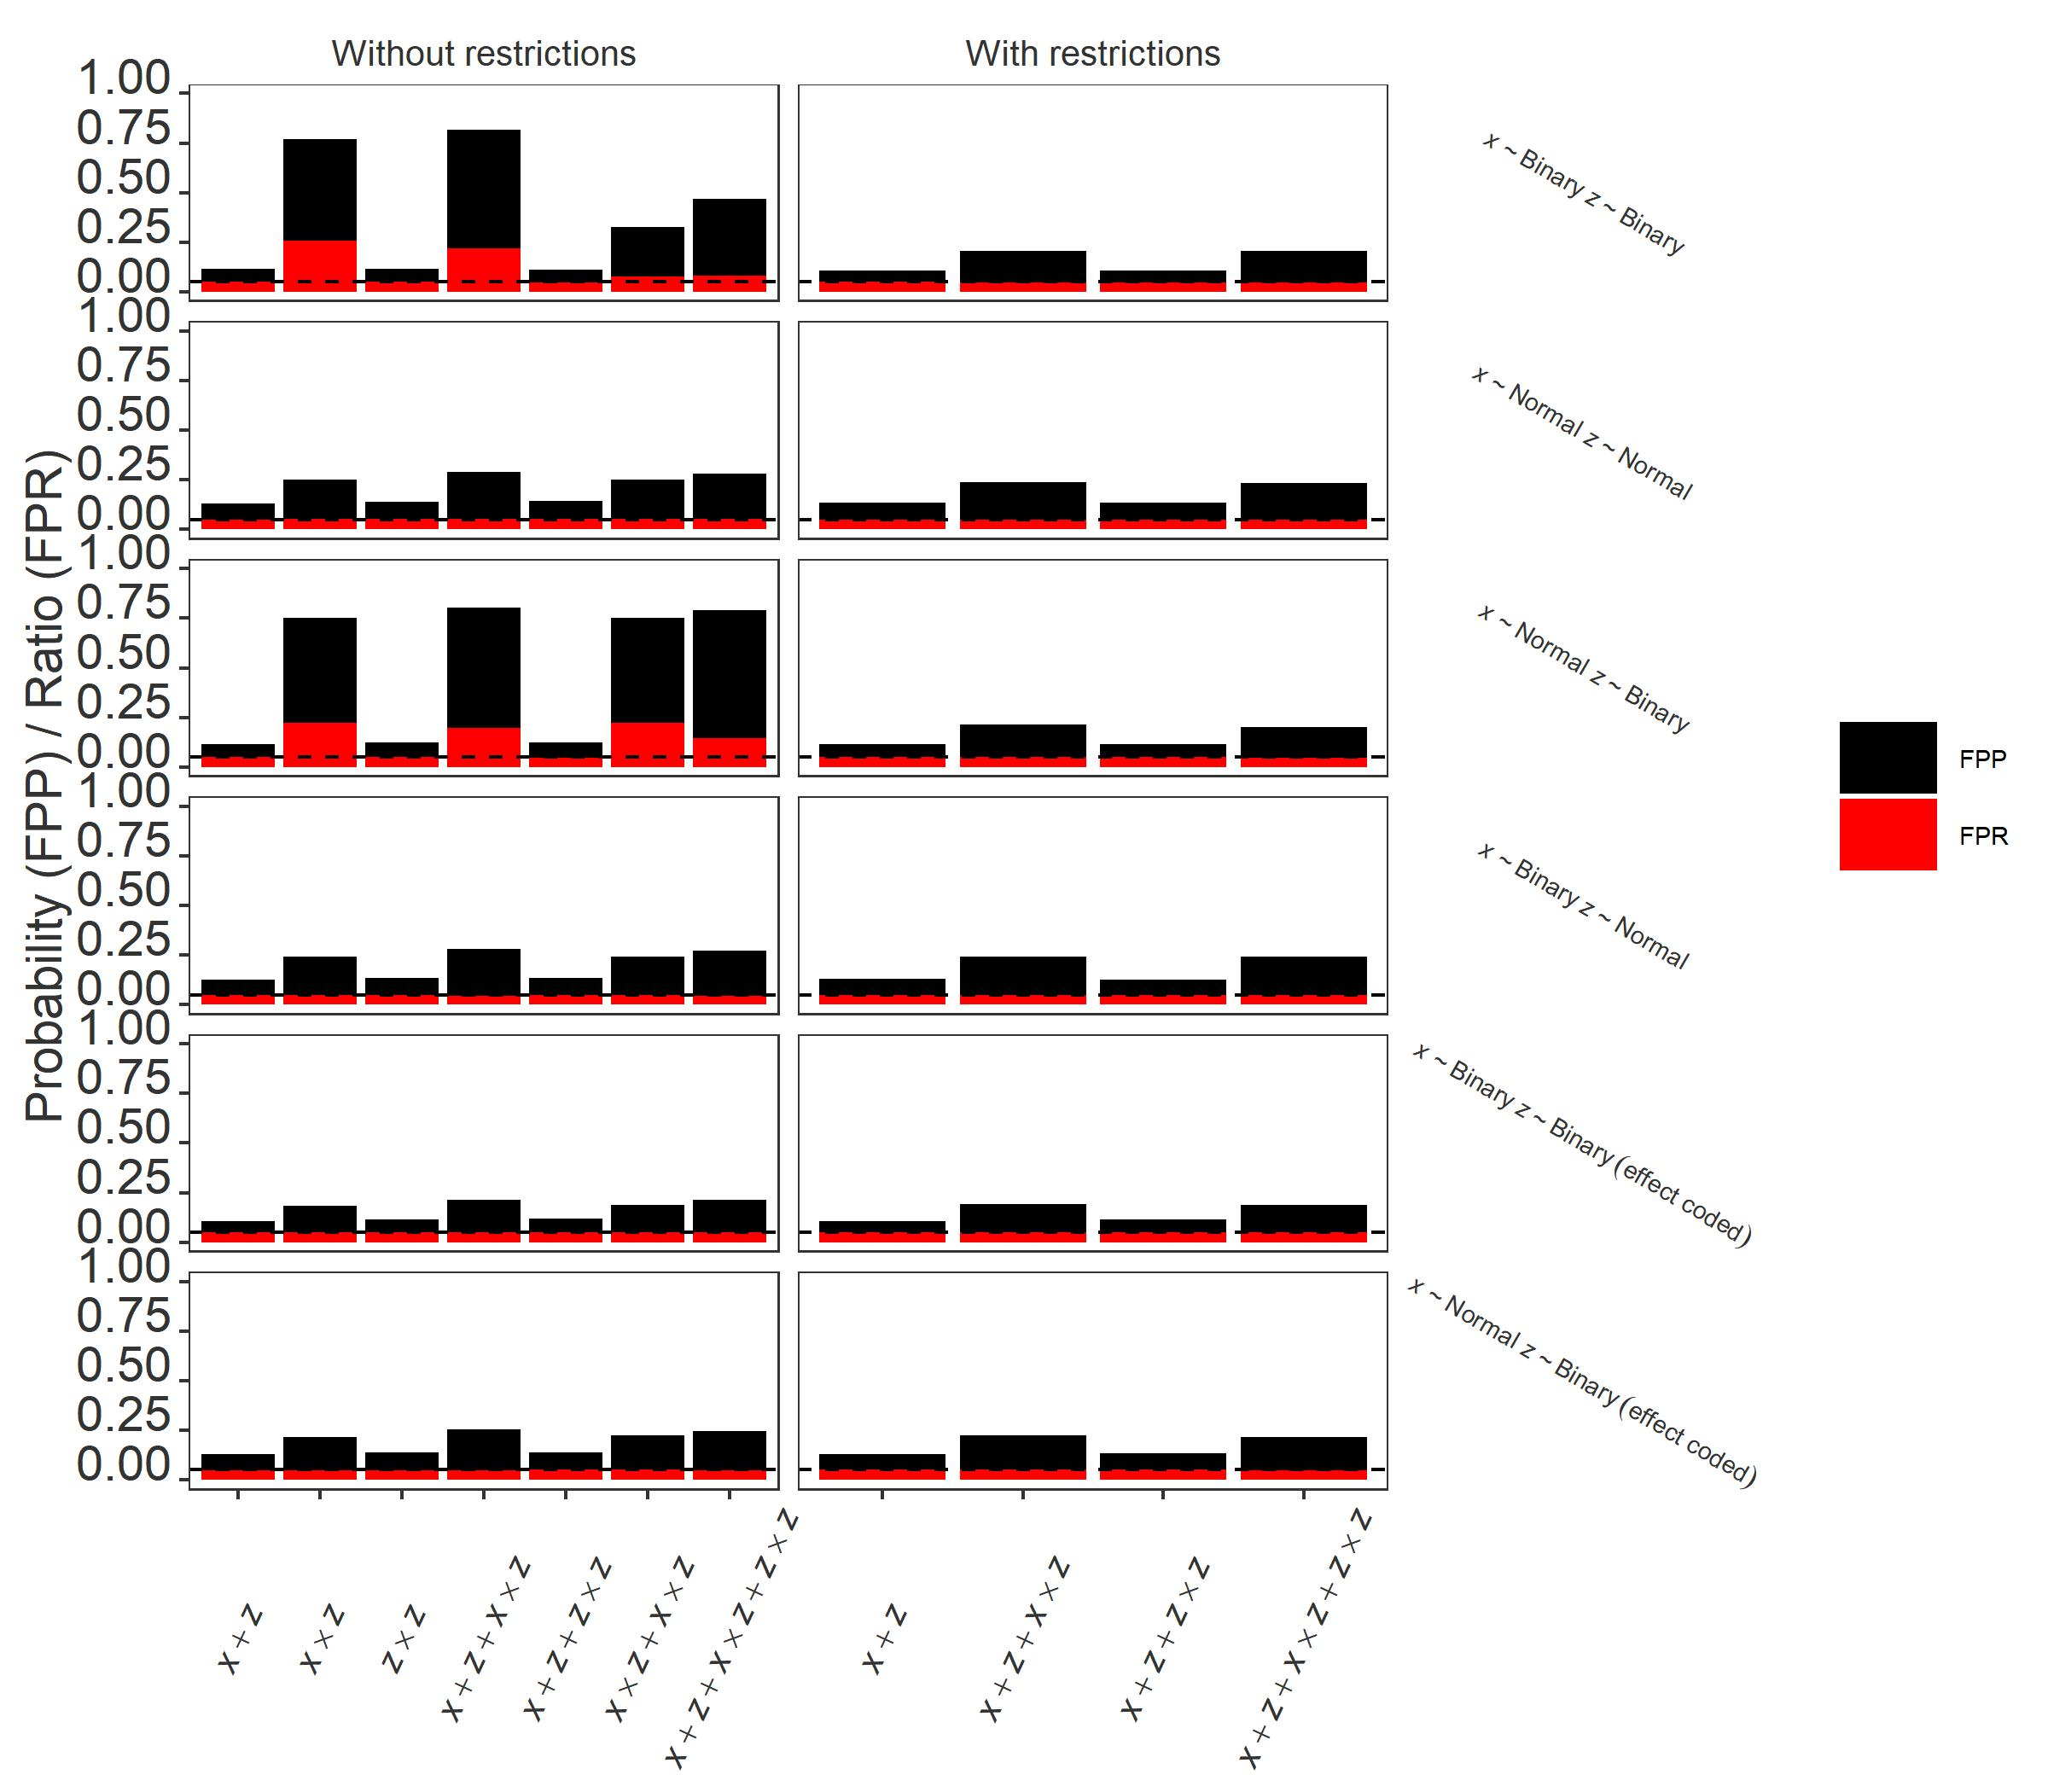
\includegraphics[scale=0.95]{R/Analysis/Result/Figures/Figure1BSIBon.jpeg}
\centering
\caption{False positive probability and false positive ratio when using multiple outlier criteria. Black denotes the the false positive probability and red denotes the false positive ratio. The description of the figure is otherwise the same as for Figure S7.
}
\label{fig:mainfigure}
\end{figure}

\begin{figure}[hbt!]
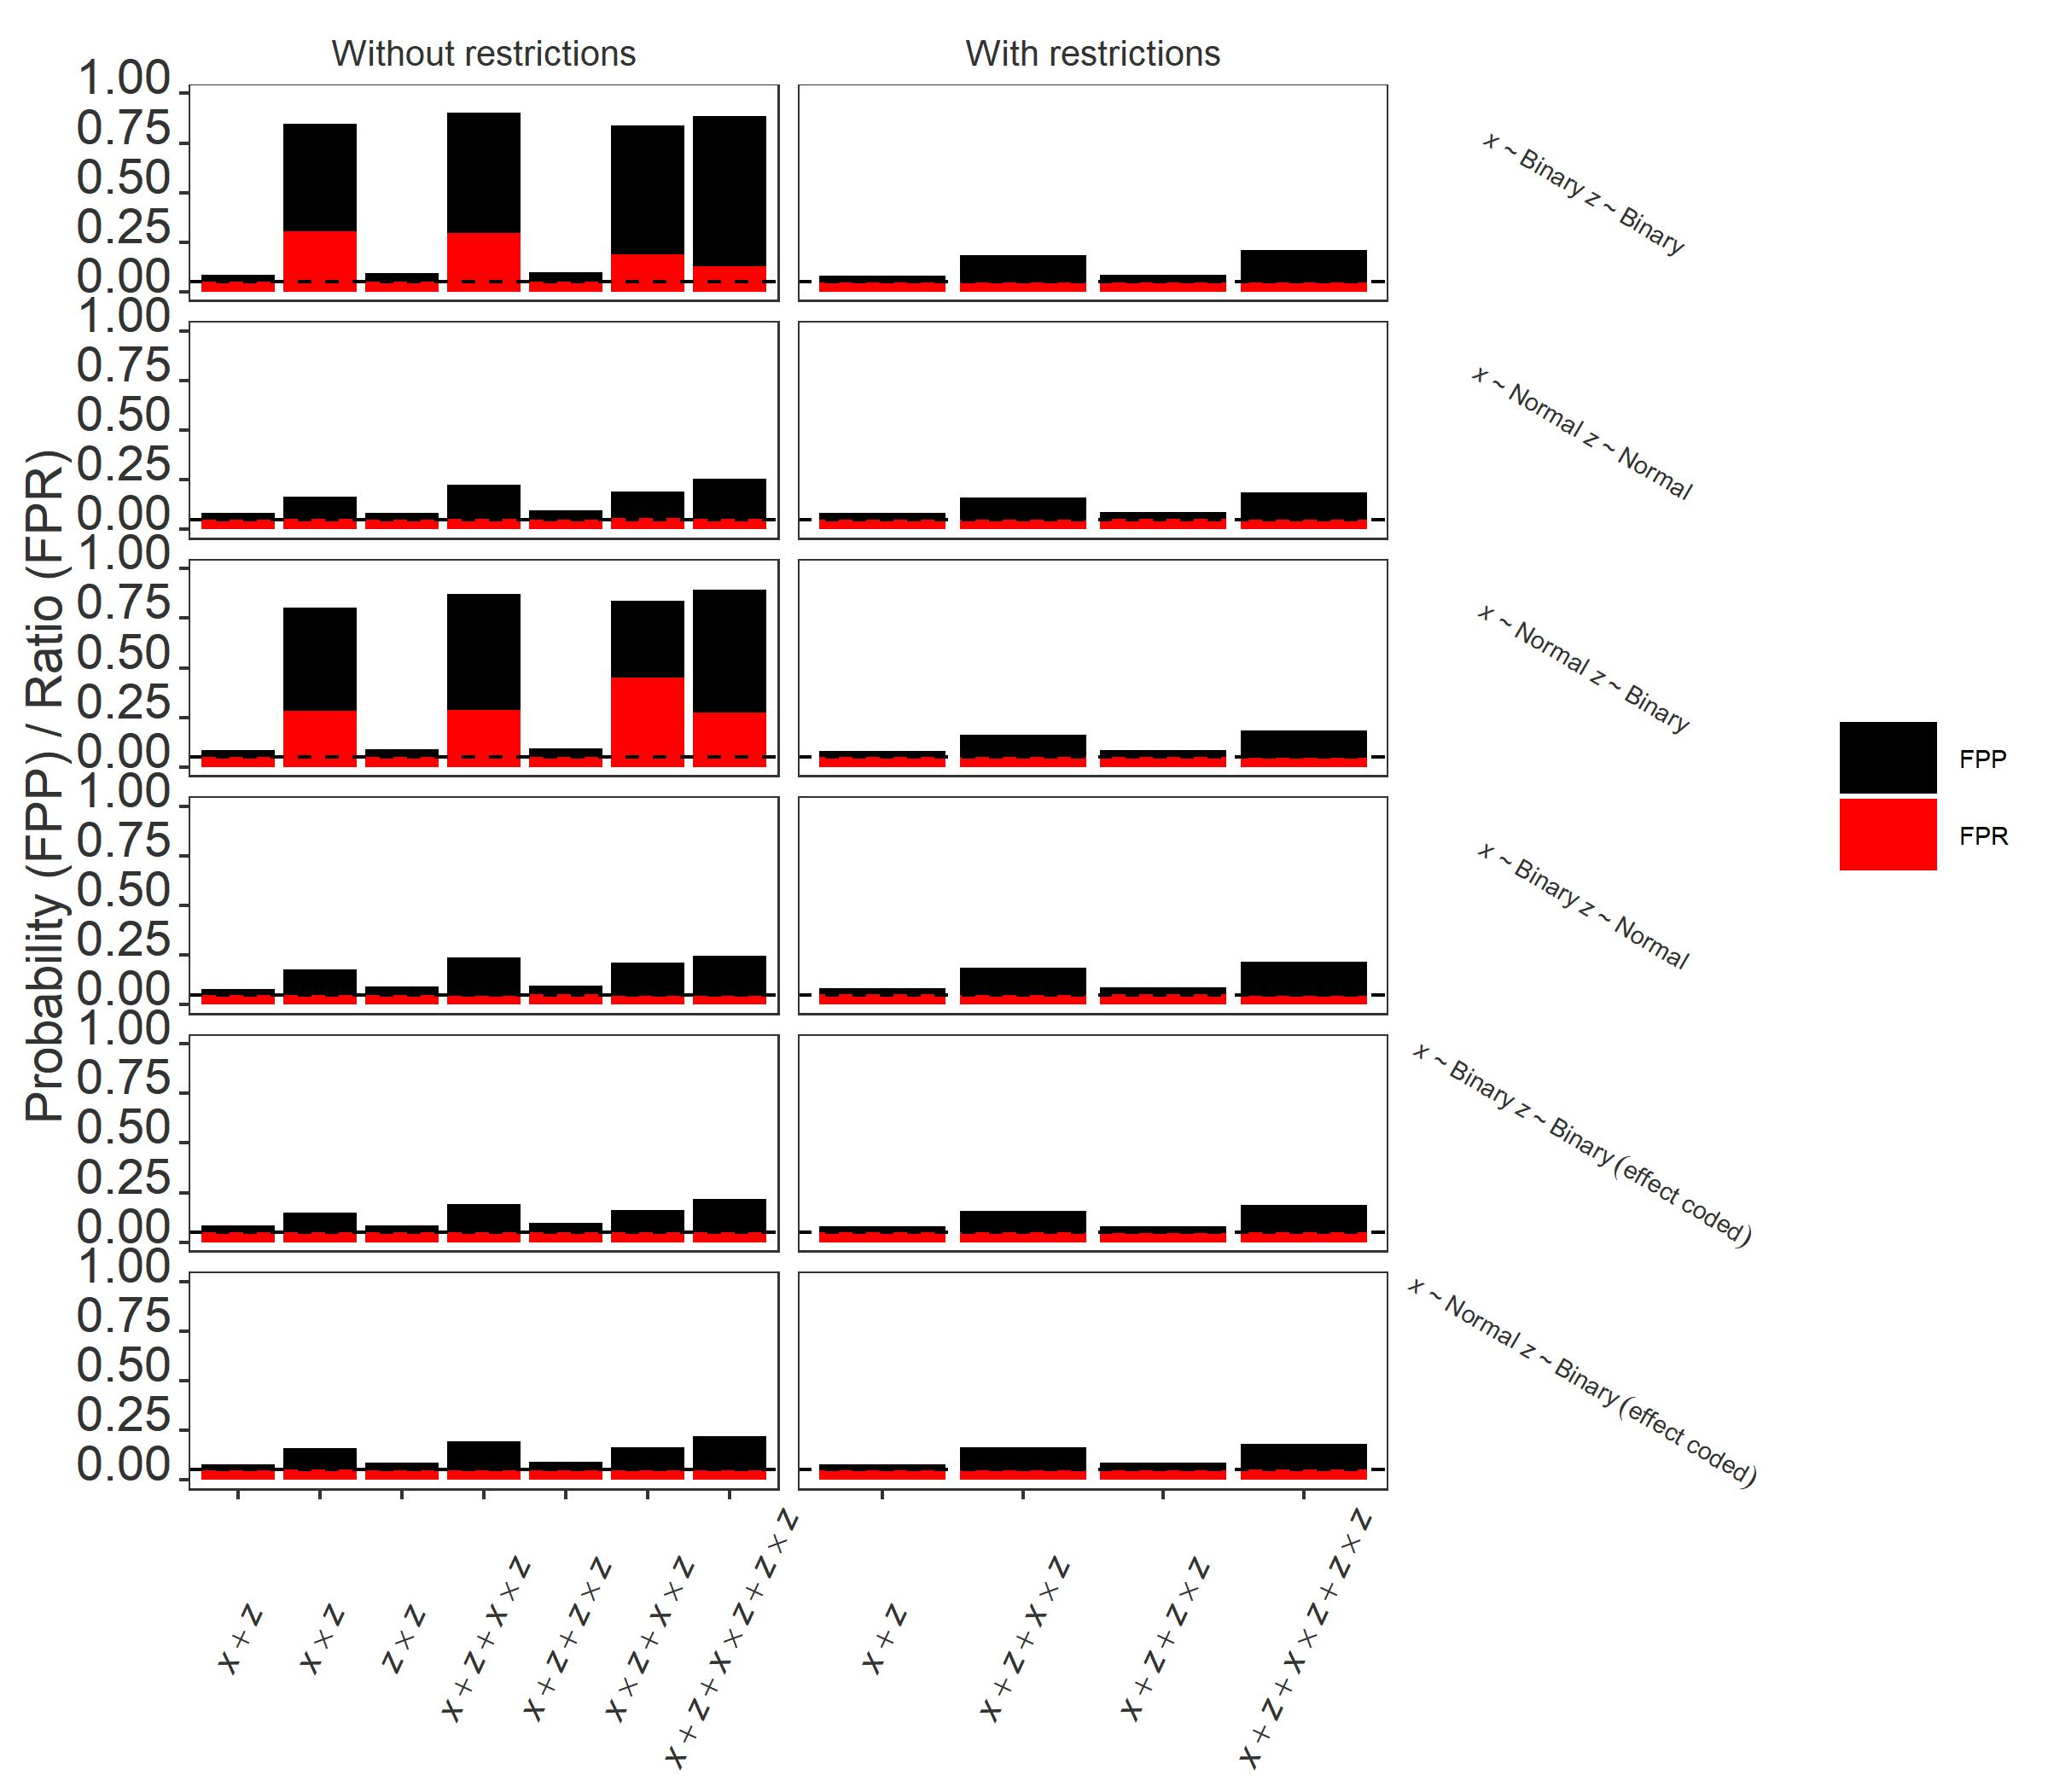
\includegraphics[scale=0.95]{R/Analysis/Result/Figures/Figure1CSIBon.jpeg}
\centering
\caption{False positive probability and false positive ratio when using three covariates instead of two as in the base line model. Black denotes the the false positive probability and red denotes the false positive ratio. The description of the figure is otherwise the same as for Figure S7.
}
\label{fig:mainfigure}
\end{figure}

\begin{landscape}
\begin{figure}[hbt!]
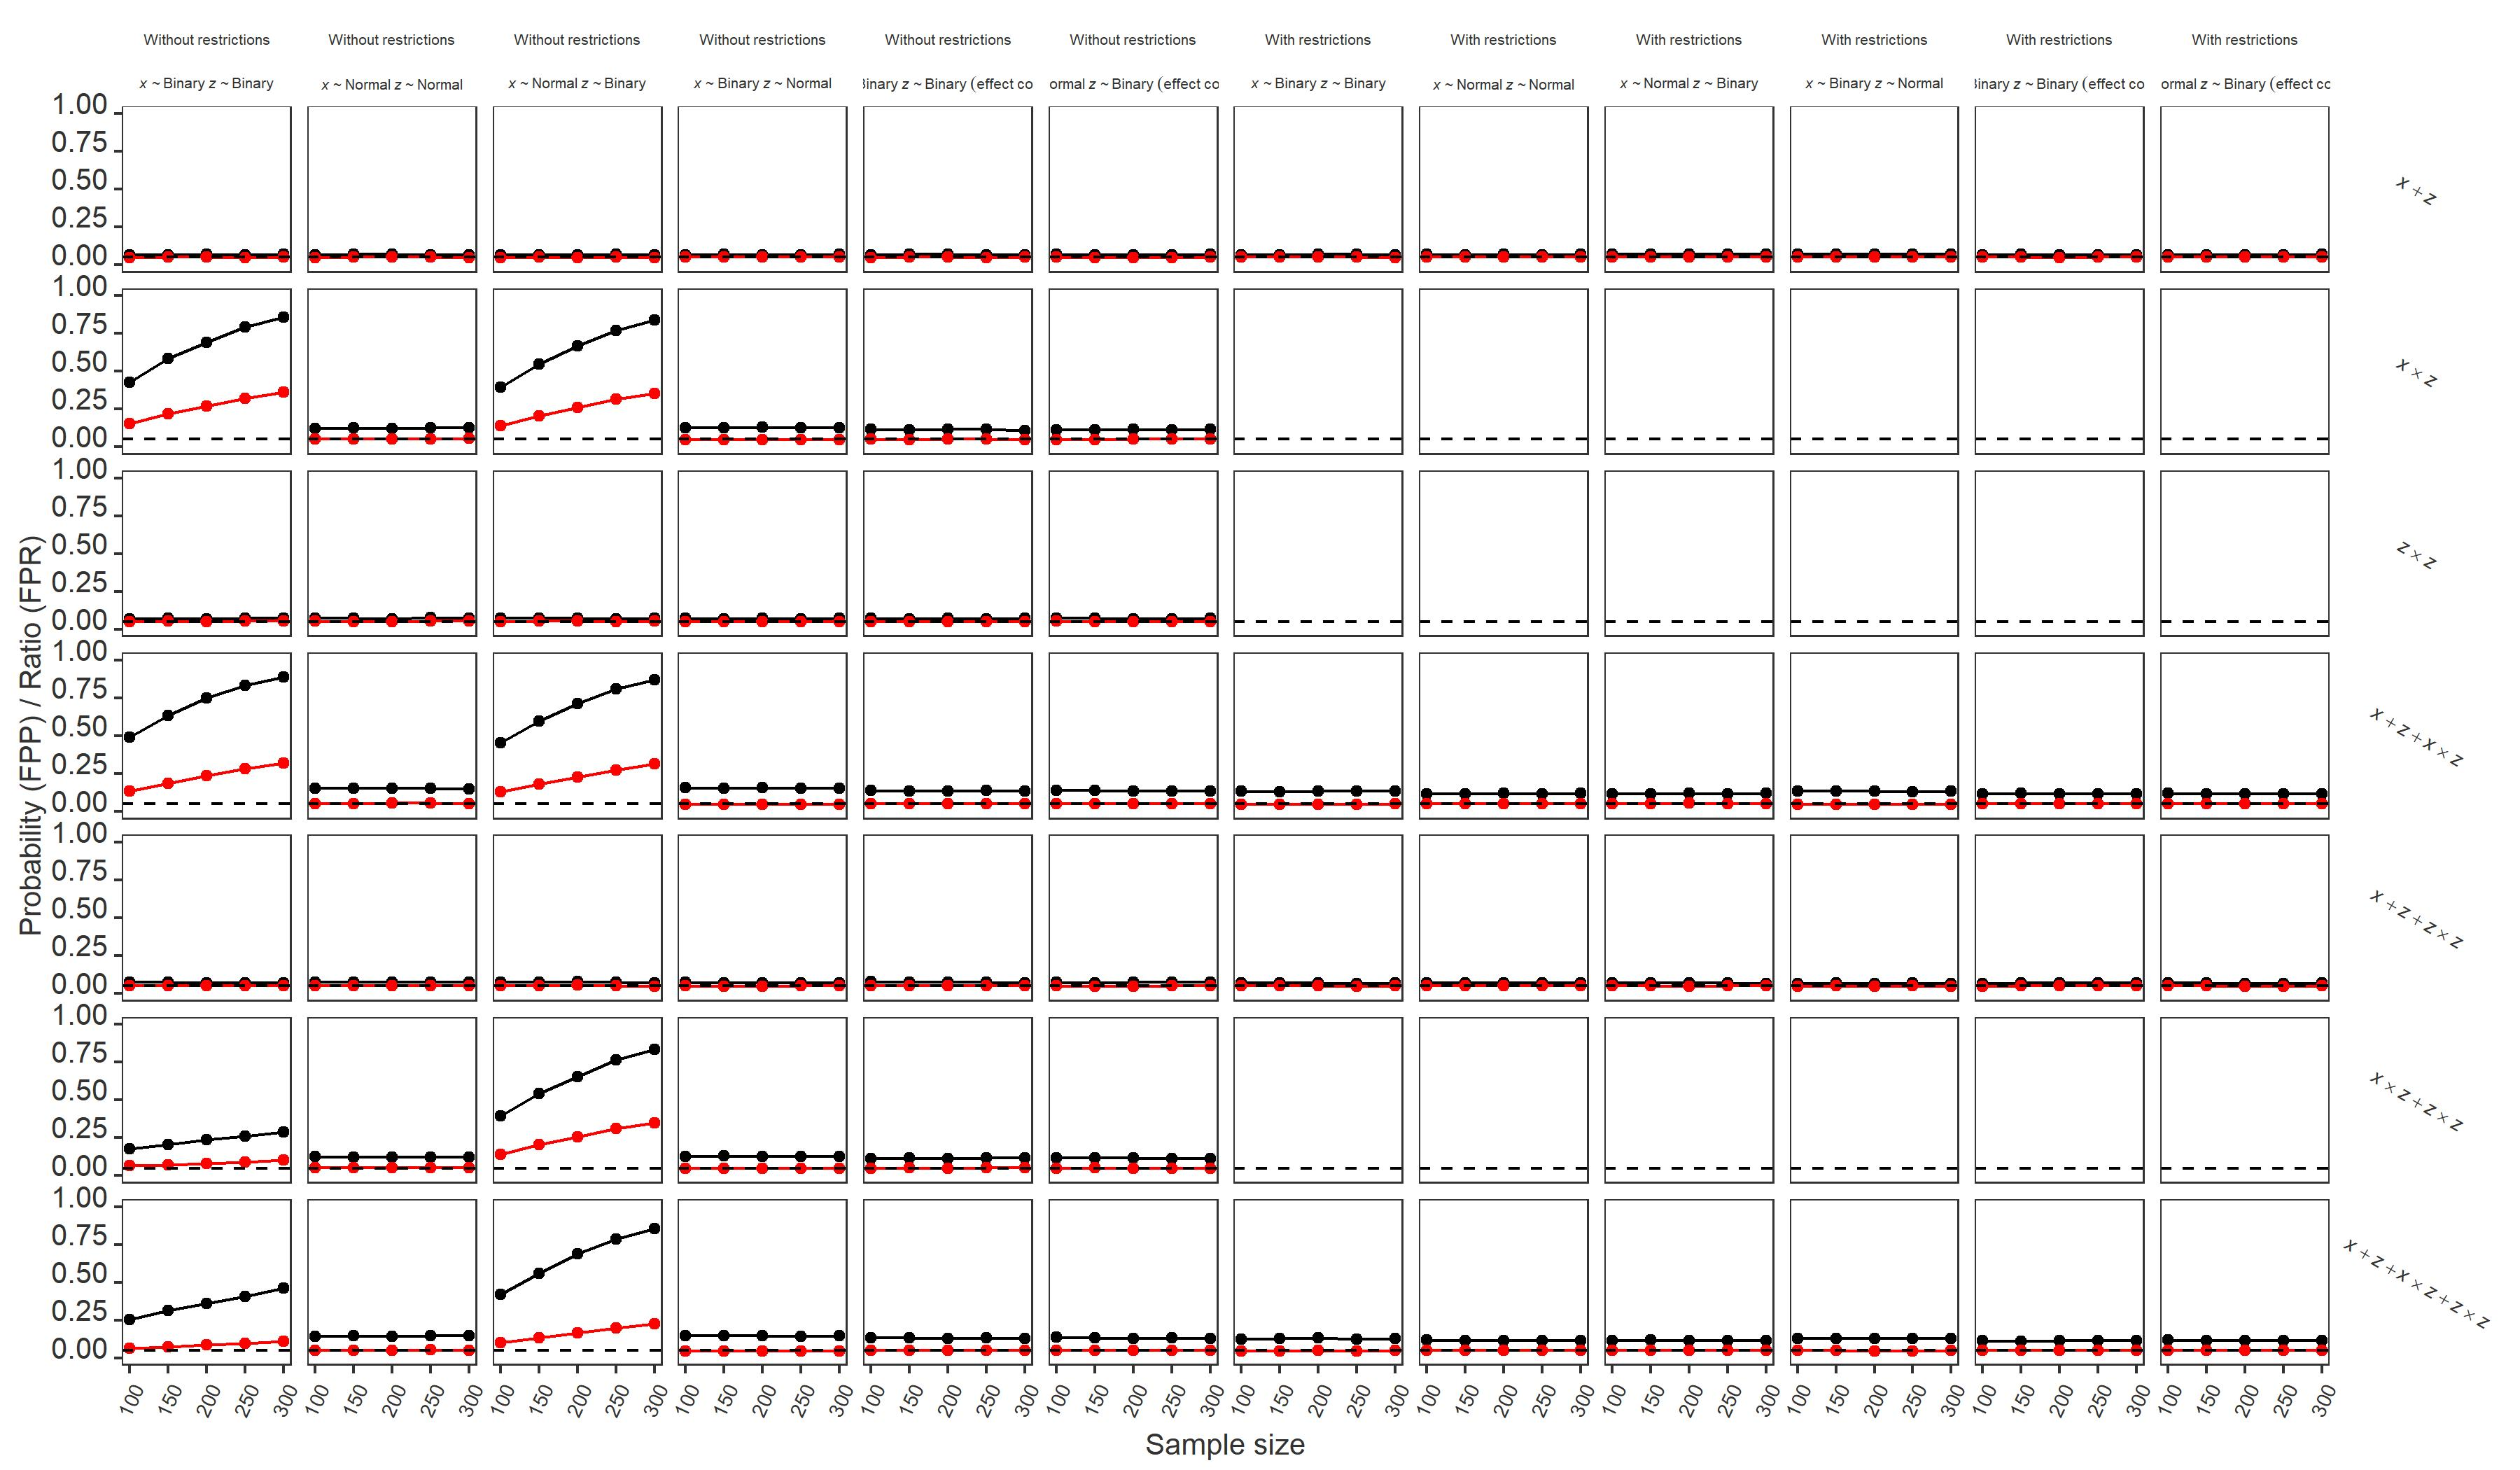
\includegraphics[scale=0.75]{R/Analysis/Result/Figures/Figure1DSIBon.jpeg}
\centering
\caption{Effect of increasing sample size for each model set and all combinations of data distributions (i.e., binary and normal) when using Bonferroni correction. Black denotes the false positive probability and red denotes the false positive ratio. The description of the figure is otherwise the same as for Figure S1.}
\label{fig:mainfigure}
\end{figure}
\end{landscape}
